\documentclass{article}
\usepackage[utf8]{inputenc}
%\usepackage{hyperref}
\usepackage[english]{babel}
\usepackage{color}
\usepackage[colorinlistoftodos]{todonotes}
\usepackage{amsmath,amssymb,amsfonts}
\usepackage{amsthm}
\usepackage{enumerate}
\usepackage{enumitem}
\usepackage{array}
\usepackage{multicol}
\usepackage[numbered,framed]{matlab-prettifier}
\usepackage{parskip}
\usepackage{subfiles}
\usepackage[toc,page]{appendix}
\usepackage{graphicx}
\usepackage{titlepic}
\usepackage{wrapfig}
\usepackage{float}
\usepackage{cite}
\usepackage{tabu}
\usepackage{amsfonts}
\usepackage{listings}
\usepackage{tikz}
\usetikzlibrary{matrix,calc}
\usepackage[nottoc]{tocbibind}
\usepackage{textcomp}
\usepackage{xcolor}
\usepackage{epstopdf}
\usepackage{caption}
\usepackage{booktabs}
\usepackage{gensymb}
\usepackage[compact]{titlesec}
\usepackage{fancyvrb}
\usepackage{eurosym}
\usepackage{soul}
\usepackage{longtable}
\usepackage[margin=1in]{geometry}
\pagestyle{plain}
%\usepackage[a4paper, total={7in, 10in}]{geometry}  Dit is voor mee text p.pag
\usepackage{hyperref}
\usepackage{import}
\usepackage[utf8]{inputenc}
\usepackage{subcaption}
\definecolor{mygreen}{RGB}{28,172,0} 
\definecolor{mylilas}{RGB}{170,55,241}
%\usepackage{lscape}
\usepackage{multirow}
\usepackage[absolute,overlay]{textpos}
\newtheorem{theorem}{Theorem}
\newtheorem{definition}{Definition}
\newtheorem{example}{Example}
\setcounter{MaxMatrixCols}{13}
\newcommand{\doctitle}{Memory Saving Multi-Observer}
\newcommand{\docsubtitle}{A Comparative Analysis of Multi-Observer Architectures for Secure State Estimation}
\newcommand{\me}{Julian Gootzen}
\newcommand{\version}{Final version}
\newcommand{\placeMonthYear}{Eindhoven, January 2025}
\newcommand{\department}{Department of Mechanical Engineering}
\newcommand{\group}{Dynamics and control}
\newcommand{\firstCommitteeMember}{dr. Michelle Chong} % use all the titles for 

\newcommand{\cJ}{|\mathcal{J}|}
\newcommand{\cP}{|\mathcal{P}|}
\newcommand{\pamu}{\texttt{pm}}
\newcommand{\mcJ}{\mathcal{J}}
\newcommand{\mcP}{\mathcal{P}}
\newcommand{\mcO}{\mathcal{O}}
\newcommand{\B}{\mathcal{B}}
\newcommand{\A}{\mathcal{A}}

% matlab parula colors
\definecolor{parula1}{rgb}{0.2422, 0.1504, 0.6603}
\definecolor{parula2}{rgb}{0.2021, 0.4788, 0.9911}
\definecolor{parula3}{rgb}{0.0704, 0.7457, 0.7258}
\definecolor{parula4}{rgb}{0.9184, 0.7308, 0.3890}
\definecolor{parula5}{rgb}{0.9769,    0.9839,    0.2805}

%\usepackage{tocloft}

\begin{document}
\lstset{language=Matlab,
	basicstyle = \scriptsize,
    breaklines=true,
    morekeywords={matlab2tikz},
    keywordstyle=\color{blue},
    morekeywords=[2]{1}, keywordstyle=[2]{\color{black}},
    identifierstyle=\color{black},
    stringstyle=\color{mylilas},
    commentstyle=\color{mygreen},
    showstringspaces=false,
    numbers=left,
    numberstyle={\small \color{black}},
    numbersep=9pt, 
    emph=[1]{for,end,break},emphstyle=[1]\color{red},   
}


\begin{titlepage}
\begin{center}

\includegraphics[height=2cm]{report/Figures/tuelogo.png}\\
%\LARGE
%Eindhoven University of Technology \\
\large
\mbox{}\department\\\mbox{}\group

\vspace*{10cm}

\setlength{\TPHorizModule}{1mm}
\setlength{\TPVertModule}{\TPHorizModule}
% Set the Paragraph Indent to zero, so the first line is not Indented
% Back-up the current value so it can be put back at the end of the title page
\newlength{\backupparindent}
\setlength{\backupparindent}{\parindent}
\setlength{\parindent}{0mm}			
% Begins a textbox at 72 mm from the left of the edge of the paper and 89 mm from the top
% The width of the textbox is 95 mm (167 - 72 mm)
% The height of the box cannot be defined, so it is your task to keep the text not too long
\begin{textblock}{95}(62,89)
    \vspace*{1mm}
    \huge
    \textbf{\doctitle \\}
    \Large
    \vspace*{5mm}
    \textit{\docsubtitle}\\
    \vspace*{10mm}
    \Large
    \me\\
    Student number: 1676512
\end{textblock}

\large
Supervisor:\\
\begin{tabular}{r}
    \mbox{}\firstCommitteeMember\\
\end{tabular}

\vfill
\version

\vfill
%\docdate \\
\large
\placeMonthYear\\

% Put the Paragraph Indent back to its original value
\setlength{\parindent}{\backupparindent}
\end{center}
\end{titlepage} 
\normalsize


\newpage
\tableofcontents\thispagestyle{empty}

\newpage
\section{Problem Statement}
Cyber physical systems (CPSs) are physical systems that are controlled by computer algorithms, actuator input is based on sensors that measure the state of the physical system. CPSs are often large, geographically dispersed, safety-critical systems that play a crucial role in modern infrastructure, such as power grids or water distribution systems. There are two categories in which most cyberattacks on CPSs can be classified: Denial of Service attakcs (DoS) and deception attacks \cite{Ding2021SecureSurvey}. A DoS attack aims to consume a significant amount of the victims resources: CPU cycles, memory bandwith or network bandwidth. The victim is then not able to use these resources for the intended purpose, for CPSs this often means that sensors do not provide any readings \cite{Yu2014AnAttacks}. A deception attack aims to completely take over a sensor, the attacker injects false data into the system \cite{Serpanos2022FalseSystems}. A deception attack is also known as a false data injection (FDI) attack. A system that is under an FDI attack still takes readings from the attacked sensor and makes decisions based on those readings. An FDI attack cannot only cause disruption of service, it can inject false data that aims to maximize long term damage to a system. 

These types of attacks on CPSs can have severe consequences on our (industrial) infrastructure. The Industroyer and Stuxnet attacks serve as infamous examples \cite{Kushner2013TheStuxnet}\cite{Lameiras2022Industroyer:Grid}. Stuxnet first lay dormant recording normal operating conditions, later it would manipulate the sensor data and cause damage to the industrial equipment. During the periods that Stuxnet manipulated sensors, it would replay the recorded data which was sent to the verification systems and were thus unaware of any abnormal operating conditions \cite{Fidler2011Was_Stuxnet_an_Act_of_War_Decoding_a_Cyberattack}. There are a number of strategies that can be employed to prevent such an attack, for example: preventing a malicious actor from gaining access to your system in the first place. Another approach, the focus of this report, is designing a system that is robust with respect to attacks. 

The control systems within CPSs often need information about all state variables used to describe the system. Measuring all state variables can be expensive, impractical or even impossible \cite{yappa}. An observer or state estimator can be used to create an estimate of all state variables from the subset of measured state variables. Considering the possible attacks on these systems, it is desirable to have the ability of providing a secure state estimate: a correct state estimate constructed from a set of noisy sensors under attack \cite{Shoukry2017SecureApproach}. This problem is also known as secure state estimation (SSE). There are several approaches to achieve SSE, such as \textcolor{red}{find a few approaches.}

This report will focus on the SSE method presented in \cite{Chong2015ObservabilityAttacks} and \cite{Chong2020AAttacks}, where an observer-based estimator is introduced. Multiple observers are created and observe the system besides each other, such an observer will be referred to as a \textit{conventional multi-observer} (CMO) in this report. This approach has an implementation bottleneck due to the large number of observers required to provide SSE, requiring large amounts of memory. A strategy to reduce memory usage is presented in \cite{Chong2023MemoryAlgorithms}, where a common state is shared between all observers. An observer with this architecture will be referred to as a \textit{state-sharing multi-observer} (SSMO). 

This BEP aims to implement both a CMO and an SSMO, compare their performance and implement an SSMO in a SSE context. In Chapter \ref{ch:system-definition} a mass-spring-damper system will be introduced. This system will serve as a case study, all MOs that are implemented in this report are applied to this system. Chapter \ref{ch:state-estimation} will introduce some important concepts fundamental principles regarding state estimation that are required to implement MOs. The CMO and SSMO will be introduced in Chapters \ref{ch:cmo} and \ref{ch:ssmo} respectively. Details of the implementation(s) will be discussed in Chapter \ref{ch:matlab-implementation}
\newpage
\section{System definition}\label{ch:system-definition}
Let us define the following continuous nonlinear time invariant multiple-input multiple-output system:
\begin{equation}\label{eqn:standard-system}
    \begin{split}
        \dot{x}(t) &= Ax(t) + Bu(t) + E\phi(x) \\
        y_i(t) &= C_ix(t) + Du(t) + v_i(t) + \tau_i(t) \quad i \in \mathcal{N} = \{1,2,\dots,N\}.
    \end{split}
\end{equation}
Where $x \in \mathbb{R}^{n_x}$, $y \in \mathbb{R}^{n_y}$, $u \in \mathbb{R}^{n_u}$ and the nonlinearity $\phi(x) \in \mathbb{R}^{n_{\phi}}$. The $(t)$ indicating time dependency will be omitted from now on. Each $i$ indicates a single output, so each $y_i$ corresponds to a $C_i \in \mathbb{R}^{1 \times n_x}$. The variables without subscript $y$ and $C$, denote all $y_i$ and $C_i$ stacked on top of each other 
$y = 
\begin{bmatrix}
    y_1 & y_2 & \cdots & y_{i} \\
\end{bmatrix}^{T}$ and
$C =
\begin{bmatrix}
    C_1^T & C_2^T & \cdots & C_i^T \\
\end{bmatrix}^{T}$
Let us consider the scenario where an attacker attacks a number of outputs $y_i$, gaining full control the attack signal $\tau_i$. No assumptions are made about $\tau_i$, it can be any unbounded signal. Let us denote the set of attacked outputs as $\mathcal{M} \subset \mathcal{N}$. \\

\subsection{Case study: multi-mass-spring-damper system}
Let us now introduce the system that will be used as a case study: a mass-spring-damper system. This system consists of $b$ mass-spring-dampers in series. Where $x_a,a=1,2,\dots,b$ denotes the position with respect to the previous mass. So the position of a block with respect to the fixed-world is
\begin{equation}\label{eqn:mass-position-wrt-fixed-world}
    \sum^{a}_{j=1}x_j.
\end{equation}
The other variables denote the following: $k_a$ is the spring constant, $c_a$ is the damping constant and $F_a$ is a force acting on the mass.
\begin{figure}[h]
    \centering
    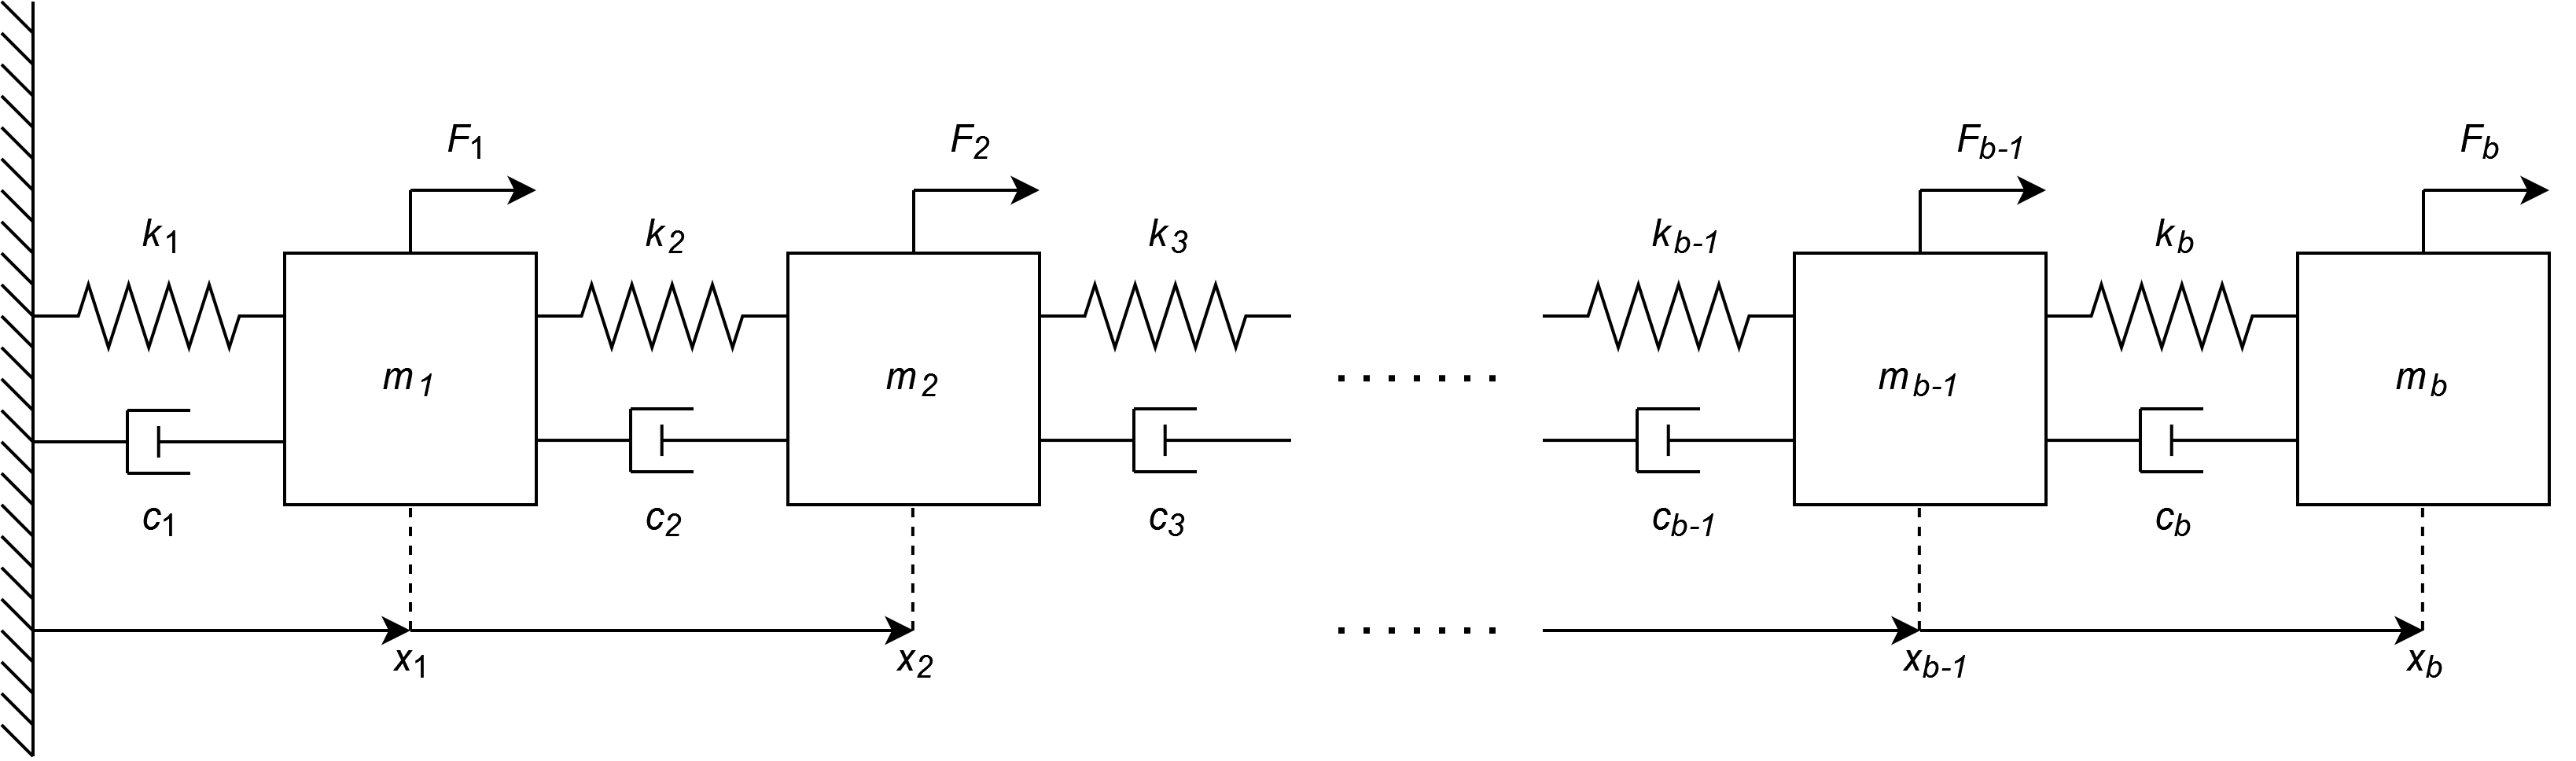
\includegraphics[width=0.9\linewidth]{report/Figures/Mass-spring-damper system.png}
    \caption{Multi-mass-spring-damper system for $b$ mass-spring-dampers in series.}
    \label{fig:mass-spring-damper-system-series}
\end{figure}

We will now derive the state-space form of the system as drawn in \autoref{fig:mass-spring-damper-system-series}. We will start by deriving the equation of motion for the first $b-1$ masses. The sum of forces on a single mass is
\begin{equation}\label{eqn:free-body-equation}
    m_a\ddot{x}_a = F_a - F_s(x_a,k_a,\eta_a) - F_d(\dot{x}_a,c_a) + F_s(x_{a+1},k_{a+1},\eta_{a+1}) + F_d(\dot{x}_{a+1},c_{a+1}).
\end{equation}
Let us now define the spring and damping forces $F_s(x_a)$ and $F_d(\dot{x}_a)$ respectively
\begin{equation*}
    F_s(x_a,k_a,\eta_a) = k_ax_a + k_a \eta_a^2 x_a^3, \quad F_d(\dot{x}_a,c_a) = c_a\dot{x}_a.
\end{equation*}
The formula for the nonlinear spring force is taken from the hardening spring example in \cite[Section 1.2.3]{Khalil2002NonlinearSystems}, the damping force is linear. The expressions for the spring force and damping force will be written as $F_s(x_a)$ and $F_d(\dot{x}_a)$ respectively, where the constants $k_a$, $\eta_a$ and $c_a$ are implicitly passed to the function. $F_s$ will be separated into a linear and nonlinear part as
\begin{equation}\label{eqn:nonlinear-spring}
    \begin{split}
        F_s(x_a) &= F_s^L(x_a) + F_s^{NL}(x_a) \\
        F_s^L(x_a) &= k_ax_a \quad , F_s^{NL}(x_a) = k_a\eta_a^2x^3_a
    \end{split}    
\end{equation}

We will now further simplify equation \eqref{eqn:free-body-equation}, with the split up $F_s$ as in equation \eqref{eqn:nonlinear-spring}

\begin{equation*}
    m_1\Ddot{x}_1 = u_1 - k_1x_1 - c_1\dot{x}_1 + k_2x_2 + c_2\dot{x}_2 - F_s^{NL}(x_1) + F_s^{NL}(x_2), \quad u_1 = F_1,
\end{equation*}
which can be rewritten into
\begin{equation}\label{eqn:mass-spring-damper-first-mass-eom}
    \Ddot{x}_1 = -\frac{k_1}{m_1}x_1 -\frac{c_1}{m_1}\dot{x}_1 + \frac{k_2}{m_1}x_2 + \frac{c_2}{m_1}\dot{x}_2 + \frac{u_1}{m_1} - \frac{F_s^{NL}(x_1)}{m_1} + \frac{F_s^{NL}(x_2)}{m_1}.
\end{equation}
Doing this for the second mass gives the following result:
\begin{equation*}
    \Ddot{x}_2 = -\frac{k_2}{m_2}x_2 - \frac{c_2}{m_2}\dot{x}_2 + \frac{k_3}{m_2}x_3 + \frac{c_3}{m_2}\dot{x}_3 + \frac{u_2}{m_2} - \frac{F_s^{NL}(x_2)}{m_1} + \frac{F_s^{NL}(x_3)}{m_1}.
\end{equation*}
which can be generalised into
\begin{equation}\label{eqn:mass-spring-damper-centre-mass-eom}
    \Ddot{x}_a =  -\frac{k_a}{m_a}x_a - \frac{c_a}{m_a}\dot{x}_a + \frac{k_{a+1}}{m_a}x_{a+1} + \frac{c_{a+1}}{m_a}\dot{x}_{a+1} + \frac{u_a}{m_a} - \frac{F_s^{NL}(x_a)}{m_a} + \frac{F_s^{NL}(x_{a+1})}{m_a}.
\end{equation}
which holds for $a \in \{2,3,\dots,b-2,b-1\}$. Now only the last mass remains
\begin{equation}\label{eqn:mass-spring-damper-last-mass-eom}
    \Ddot{x}_b = -\frac{k_b}{m_b}x_b - \frac{c_b}{m_b}\dot{x}_b + \frac{u_b}{m_b} - \frac{F_s^{NL}(x_b)}{m_b}
\end{equation}

Let us now define the state vector $x$ from equation \eqref{eqn:standard-system} as
\begin{equation}\label{eqn:msd-x}
    x =
    \begin{bmatrix}
        x_1 & \dot{x}_1 & x_2 & \dot{x}_2 & \cdots & x_b & \dot{x}_{b}
    \end{bmatrix}^T
\end{equation}
Using equations \eqref{eqn:mass-spring-damper-first-mass-eom}\eqref{eqn:mass-spring-damper-centre-mass-eom}\eqref{eqn:mass-spring-damper-last-mass-eom} can now be used to construct the $A$ and $B$ matrices in equation \eqref{eqn:standard-system}
\begin{equation}\label{eqn:msd-A}
    A =
    \begin{bmatrix}
        0 & 1 & 0 & 0 & 0 & 0 & \cdots & 0 & 0 & 0 & 0 \\
        -\frac{k_1}{m_1} & -\frac{c_1}{m_1} & \frac{k_2}{m_1} & \frac{c_2}{m_1} & 0 & 0 & \cdots & 0 & 0 & 0 & 0 \\
        0 & 0 & 0 & 1 & 0 & 0 & \cdots & 0 & 0 & 0 & 0 \\
       0 & 0 & -\frac{k_2}{m_2} & -\frac{c_2}{m_2} & \frac{k_3}{m_2} & \frac{c_3}{m_2} & \cdots & 0 & 0 & 0 & 0 \\
        \vdots & \vdots & \vdots & \vdots & \vdots & \vdots & \ddots & \vdots & \vdots & \vdots & \vdots \\
        0 & 0 & 0 & 0 & 0 & 0 & \cdots & 0 & 0 & 0 & 1 \\
        0 & 0 & 0 & 0 & 0 & 0 & \cdots & 0 & 0 & -\frac{k_b}{m_b} & -\frac{c_b}{m_b} \\
    \end{bmatrix}
\end{equation}
and
\begin{equation}\label{eqn:msd-B}
    B = 
    \begin{bmatrix}
        0 & 0 & \cdots & 0 \\
        \frac{1}{m_1} & 0 & \cdots & 0 \\
        0 & 0 & \cdots & 0 \\
        0 & \frac{1}{m_2} & \cdots & 0 \\
        \vdots & \vdots & \ddots & \vdots \\
        0 & 0 & \cdots & 0 \\
        0 & 0 & \cdots & \frac{1}{m_b} \\
    \end{bmatrix}.
\end{equation}
Let us now derive the nonlinear contributions $\phi$ and $E$ from equation \eqref{eqn:standard-system} from equations \eqref{eqn:mass-spring-damper-first-mass-eom}\eqref{eqn:mass-spring-damper-centre-mass-eom}\eqref{eqn:mass-spring-damper-last-mass-eom}.
\begin{equation}
    \phi(x) =
    \begin{bmatrix}
        F_s^{NL}(x_1) & F_s^{NL}(x_2) & \cdots & F_s^{NL}(x_b)
    \end{bmatrix}
\end{equation}
and
\begin{equation}
    E =
    \begin{bmatrix}
        0 & 0 & 0 & \cdots & 0 \\
        -\frac{1}{m_1} & \frac{1}{m_1} & 0 & \cdots & 0 \\
        0 & 0 & 0 & \cdots & 0 \\
        0 & -\frac{1}{m_2} & \frac{1}{m_2} & \cdots & 0 \\
        \vdots & \vdots & \vdots & \ddots & \vdots \\
        0 & 0 & 0 & \cdots & 0 \\
        0 & 0 & 0 & \cdots & -\frac{1}{m_b} \\
    \end{bmatrix}.
\end{equation}

We will now construct the $C$ matrix, in order to do so let us note that only the absolute positions \eqref{eqn:mass-position-wrt-fixed-world} of each mass are measured. This leads to
\begin{equation}\label{eqn:msd-C}
    C = 
    \begin{bmatrix}
        1 & 0 & 0 & 0 & \cdots & 0 & 0 & 0 & 0 \\
        1 & 0 & 1 & 0 & \cdots & 0 & 0 & 0 & 0 \\
        \vdots & \vdots & \vdots & \vdots & \ddots & \vdots & \vdots & \vdots & \vdots \\
        1 & 0 & 1 & 0 & \cdots & 1 & 0 & 0 & 0 \\
        1 & 0 & 1 & 0 & \cdots & 1 & 0 & 1 & 0 \\
    \end{bmatrix}
\end{equation}
where each row is a single output. In this system the $D$ matrix is equal to $0$.\\ 
\textcolor{red}{note on observability?}
\newpage


\section{Conventional multi-observer}
In this section the CMO will be introduced and two implementations will be discussed. Let us first further elaborate on the what the CMO should achieve. Let us look at the case where a 'single'-observer \eqref{eqn:unstable-simple-state-estimator} is employed to construct the state estimate of system \eqref{eqn:standard-system}, where $w=0$ and $v=0$. When an attacker gains control over some of the outputs $y_i$ and attacks it with the attack signal $\tau_i$. Performing the same analysis on the derivative of error \eqref{eqn:estimate-error} leads to
\begin{equation*}
    \begin{split}
        \dot{e} = \dot{\hat{x}} - \dot{x} &= A\hat{x} + Bu + E\phi(y) + L(C\hat{x} - Cx - \tau) - Ax - Bu - E\phi(y) \\
        &= (A+LC)e - L\tau,
    \end{split}
\end{equation*}
which does not guarantee $e \rightarrow 0$ as $t \rightarrow \infty$. The CMO aims to still provide a correct state estimate even when a subset $\mathcal{M} \subset \mathcal{N}$ outputs are under attack, where $2|\mathcal{M}| < |\mathcal{N}|$. 

\subsection{Constructing the state estimates}
\label{subsec:state-estimates}
The multi-observer described in this section is based on \cite[III B]{Chong2015ObservabilityAttacks}. This CMO is able to correctly estimate the state when up to $N_M = |\mathcal{M}|$ outputs are under attack. $N_M$ is required to satisfy $2N_M<N_O$, in other words: more than half the sensors need to remain attack free at all times. Consider system \eqref{eqn:standard-system} with $N_O$ outputs
\begin{equation*}
    \begin{split}
    \dot{x} &= Ax + Bu + E\phi(y) + w \\
        y_i &= C_ix + Du + v_i + \tau_i \quad i  \in \{1,2,\dots,N_O\}.
    \end{split}
\end{equation*}
Let us define $\mathcal{J} \subset \{1,2,\dots,N\}$ and $\mathcal{P} \subset \{1,2,\dots,N\}$ as all sets with  $J=N_O-N_M$ and  $P=1$ elements respectively. $P$ could also be taken as any value smaller than $J$, we restrict ourselves to systems that are fully observable trough any single output $y_i = C_ix$. The cardinalities of $\mathcal{J}$ and $\mathcal{P}$ are 
\begin{equation}\label{eqn:multi-observer-sizes}
    N_J = \cJ={N_O \choose J}={N_O \choose N_O-N_M}, \quad N_P = \cP = {N_O \choose P} = N_O.
\end{equation}
For example, $N_O=17$ and $N_M=8$ ($N_O>2N_M$) leads to $N_J=24310$ and $N_P=17$.
We now define the $j=1,2,\dots,N_J$ $J$\textit{-observers} as
\begin{equation*}
    \begin{split}
        \dot{\hat{x}}_j^\mcJ &= A\hat{x}_j^\mcJ + Bu + E\phi(y) + L_j(\hat{y}_j^\mcJ - y_j) \\
        \hat{y}_j^\mcJ &= C_j\hat{x}_j^\mcJ + Du
    \end{split}
\end{equation*}
where $j$ is a single combination out of all outputs and $L_j$ is an output injection gain that can be chosen in such a way to place the eigenvalues at a desired location if and only if the pair $(A,C_j)$ is observable. For example when $N_O=5$ and $N_M=2$, a possible $j$ is $\{1,3,4\}$ or $\{2,3,5\}$. The $J$ in the superscript indicates that this is a variable that relates to an observer that uses $J$ out of $N_O$ outputs.
Substituting $\hat{y}_j^J$ and $y_j$ in $\dot{\hat{x}}_j^J$ leads to
\begin{equation}\label{eqn:cmo-single-J-observer}
    \begin{split}
        \dot{\hat{x}}_j^{\mcJ} &= Ax_j^{\mcJ} + Bu + E\phi(y) + L_j^{\mcJ}(C\hat{x}_j^{\mcJ} + Du - C_j^{\mcJ}x - Du - v_j^{\mcJ}) \\
        \dot{\hat{x}}_j^{\mcJ} &= (A + L_j^{\mcJ}C_j^{\mcJ})\hat{x}_j - L_j^JC_j^{\mcJ}x + Bu + E\phi(y) - L_j^{\mcJ}(v_j^{\mcJ} + \tau_j^{\mcJ}). \\
    \end{split}    
\end{equation}
Doing the same for the the $p=1,2,\dots,N_P$ $P$\textit{-observers} leads to
\begin{equation}\label{eqn:cmo-single-P-observer}
    \dot{\hat{x}}_p^{\mcP} = (A + L_p^{\mcP}C_p^{\mcP})\hat{x}_p^{\mcP} - L_p^{\mcP}C_p^{\mcP}x + Bu + E\phi(y) - L_p^{\mcP}(v_p^{\mcP} + \tau_p^{\mcP}).
\end{equation}
Where $C_p$ and $C_i$ are the rows. All observers in \eqref{eqn:cmo-single-J-observer} and \eqref{eqn:cmo-single-P-observer} form a \textit{multi-observer}. Note that for a system with $N_M$ the largest possible number so that $N_O > 2N_M$, there is exactly one possible combination with $J$ elements out of all $N_J$ possible combinations that does not contain any of the $N_M$ attacked outputs. We now need to derive a method to select this one attack free observer from all observers. That is where the $P$-observers are used.

\subsection{Final estimate selection procedure}
\label{subsec:estimate-selection}
Now that all state estimates are constructed, a 'final' estimate $\hat{x}$ needs to be selected from all $\hat{x}_j^{\mcJ}$ First, a comparison will be made between all $J$-observers and the $P$-observers that are \textit{sub-observers}, implying that all outputs used to construct the state estimate $\hat{x}_p^{\mcP}$ are also used in the state estimate $\hat{x}_j^{\mcJ}$. For example, when $N_O=4$ $N_M=1$ one of the $J$-observer uses $j=\{1,2,4\}$ as outputs. The $P$-estimates would be constructed with $p \in \{1,2,4\}$. Let us define 
\begin{equation*}
   \pi_{j} = \max_{p \subset j} |\hat{x}_{j} - \hat{x}_{p}|
\end{equation*}
so the largest difference between the $j$-estimate and its $p$-estimates, where the $p$-observers are all a sub-observers of the $j$-observer. We now collect all $\pi_j$ in
\begin{equation*}
   \pi_{\mathcal{J}} = \max_{\mathcal{P} \subset \mathcal{J}} |\hat{x}_{\mathcal{J}} - \hat{x}_{\mathcal{P}}|
\end{equation*}

where $\hat{x}_{\mathcal{J}}$ are all state estimates from \eqref{eqn:cmo-single-J-observer} and $\hat{x}_{\mathcal{P}}$ are all sub-observers off each $j \in \mcJ$. Let us now choose the smallest $\pi_J$
\begin{equation}
    \sigma = \arg \min \pi_{\mathcal{J}}, \quad \sigma \subset \{1,2,\dots,N_J\}.
\end{equation}
We can now select the final state estimate as
\begin{equation}
    \hat{x} = \hat{x}_{\sigma}.
\end{equation}
This selection procedure selects the observer which has the smallest difference between itself and its sub-observers. 

\subsection{Implementations}
The state estimates constructed in \ref{subsec:state-estimates} only serve as a basis of the CMO, in this subsection two different implementations will be discussed. These implementations will be implemented in Matlab in the next chapter \textcolor{red}{ref this shit}. The first one  stores all the observers in a 2D matrix and will thus be known as the 2D-CMO. The second implementation stores the observers in a 3D matrix and will thus be known as the 3D-CMO.

\subsubsection{2D conventional multi-observer}
\textcolor{red}{decide if I want to keep this in, would require fintuning the implementation and adding the nonlinearity}
Let us write all observers \eqref{eqn:cmo-single-J-observer}\eqref{eqn:cmo-single-P-observer} in the following form
\begin{equation*}
    \dot{\Tilde{x}}_{2D} = \Tilde{A}_{2D}\Tilde{x}_{2D} + F_{2D}\eta_{2D}
\end{equation*}
where
\begin{equation}\label{eqn:2D-CMO}
\renewcommand{\arraystretch}{1.3}
    \begin{split}    
        \Tilde{x}_{2D} &= 
        \begin{bmatrix}
            \hat{x}_1^{\mcJ} \\ \vdots \\ \hat{x}_{N_J}^{\mcJ} \\ \hat{x}_1^{P} \\ \vdots \\ \hat{x}_{N_P}^{\mcP}
        \end{bmatrix}, \quad
        \Tilde{A}_{2D} = 
        \begin{bmatrix}
            -L_1^{\mcJ}C_1^{\mcJ} & A + L_1^{\mcJ}C_1^{\mcJ} & \cdots & 0  & 0 & \cdots & 0 \\
            \vdots & \vdots & \ddots & \vdots & \vdots & & \vdots \\
            -L_{N_J}^{\mcJ}C_{N_J}^{\mcJ} & 0 & \cdots & A + L_{N_J}^{\mcJ}C_{N_J}^{\mcJ} & 0 & \cdots & 0 \\
            -L_{1}^{\mcP}C_{1}^{\mcP} & 0 & \cdots & 0 & A + L_1^{\mcP}C_1^{\mcP} & \cdots & 0 \\
            \vdots & \vdots &  & \vdots & \vdots & \ddots & \vdots \\
            -L_{N_P}^{\mcP}C_{N_P}^{\mcP} & 0 & \cdots & 0 & 0 & \cdots & A + L_{N_P}^{\mcP}C_{N_P}^{\mcP} \\
        \end{bmatrix} \\
        \eta &= 
        \begin{bmatrix}
            u \\ v_1^{\mcJ} + \tau_1^{\mcJ} \\ \vdots \\ v_{N_J}^{\mcJ} + \tau_{N_J}^J \\ v_1^{\mcP} + \tau_1^{\mcP} \\ \vdots \\ v_{N_P}^{\mcP} + \tau_{N_P}^{\mcP} \\ w \\
        \end{bmatrix}, \quad 
        F_{2D} = 
        \begin{bmatrix}
            B & -L_1^{\mcJ} & \cdots & 0 & 0 & \cdots & 0 \\
            \vdots & \vdots & \ddots & \vdots & \vdots & & \vdots \\
            B & 0 & \cdots & -L_{\cJ}^{\mcJ} & 0 & \cdots & 0 \\
            B & 0 & \cdots & 0 & -L_{1}^{\mcP} & \cdots & 0 \\
            \vdots & \vdots & & \vdots & \vdots & \ddots & \vdots \\
            B & 0 & \cdots & 0 & 0 & \cdots & -L_{N_P}^{\mcP} \\
        \end{bmatrix}\\
    \end{split}
\end{equation}
The $\Tilde{A}$ matrix stores  all $J$- and $P$-estimates: the top section stores the $J$-observers and on the bottom the $P$-observers. Multiplying this $\Tilde{A}_{2D}$ matrix by $\Tilde{x}_{2D}$ leads to the state estimators presented in \eqref{eqn:cmo-single-J-observer} and \eqref{eqn:cmo-single-P-observer} without inputs, noise and attacks. The vector $\eta$ stacks the input and sum of sensor noise and attack signal on top of each other and the matrix $E$ stores all factors that need to be multiplied with $\eta$ to arrive at \eqref{eqn:cmo-single-J-observer} and \eqref{eqn:cmo-single-P-observer}.

\newcommand{\ntwoD}{nN_S}
\begin{table}[h]
    \centering
    \begin{tabular}{c|c|c}
       Matrix  & Dimensions & Number of elements \\ \hline
       $\Tilde{x}_{2D}$  & $\ntwoD \times 1$ & $nN_S$ \\
       $\Tilde{A}_{2D}$ & $\ntwoD \times \ntwoD$ & $n^2N_S^2$ \\
       $B_{2D}$ & $k \times N_S$ & $kN_S$ \\
       $u_{2D}$ & $k \times N_S$ & $kN_S$ \\
    \end{tabular}
    \caption{2D-CMO system matrix dimensions}
    \label{tab:2D-CMO-dimensions}
\end{table}



\newpage
\subsubsection{3D conventional multi-observer}
Now the second implementation of the CMO will be discussed. The goal of the 3D-CMO is to reduce the number of zeros required in the $\Tilde{A}_{2D}$\eqref{eqn:2D-CMO}. In order to do so we store all block matrices behind each other. Let us start by defining 
\begin{center}
    \begin{minipage}[t]{0.4\textwidth}
        \centering
        % First tikzpicture
        \begin{equation}\label{eqn:x3d}
            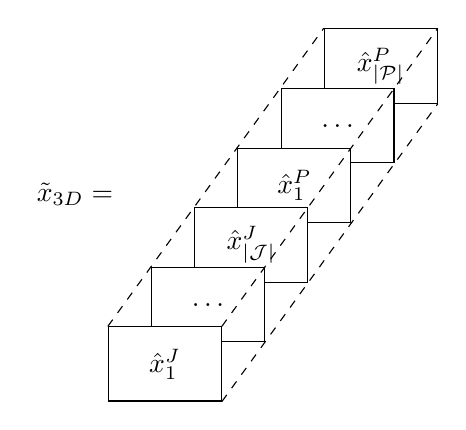
\begin{tikzpicture}[every node/.style={anchor=north east,fill=white,minimum width=1.2cm,minimum height=7mm}] 
            % Define the displacement as a coordinate
            \coordinate (displacement) at (0.9,0.2);
        
            \matrix (mxP) [draw,matrix of math nodes]
                {
                \hat{x}_{\cP}^P \\
                };
        
            \matrix (dots2) [draw,matrix of math nodes] at ($(mxP.south west)+(displacement)$)
                {
                \dots \\
                };
        
            \matrix (mxp) [draw,matrix of math nodes] at ($(dots2.south west)+(displacement)$)
                {
                \hat{x}_1^P \\
                };
        
            \matrix (mxJ) [draw,matrix of math nodes] at ($(mxp.south west)+(displacement)$)
                {
                \hat{x}_{\cJ}^J \\
                };
        
            \matrix (dots1) [draw,matrix of math nodes] at ($(mxJ.south west)+(displacement)$)
                {
                \dots \\
                };
        
            \matrix (mxj) [draw,matrix of math nodes] at ($(dots1.south west)+(displacement)$)
                {
                \hat{x}_1^J \\
                };
    
            \node at ($(-4,-1.75)$) {$\tilde{x}_{3D}=$};
            
            \draw[dashed](mxj.north east)--(mxP.north east);
            \draw[dashed](mxj.north west)--(mxP.north west);
            \draw[dashed](mxj.south east)--(mxP.south east);
    
        \end{tikzpicture}
        \end{equation}
    \end{minipage}
    \begin{minipage}[t]{0.4\textwidth}
        \centering
        % Second tikzpicture
        \begin{equation}\label{eqn:A-tilde-3D}
            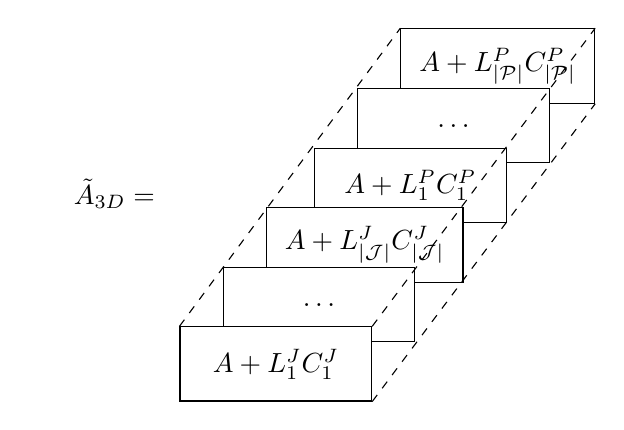
\begin{tikzpicture}[every node/.style={anchor=north east,fill=white,minimum width=2.2cm,minimum height=7mm}]
            
            % Define the displacement as a coordinate
            \coordinate (displacement) at (1.9,0.2);
        
            \matrix (mAP) [draw,matrix of math nodes]
                {
                A + L_{\cP}^PC_{\cP}^P \\
                };
        
            \matrix (dots2) [draw,matrix of math nodes] at ($(mAP.south west)+(displacement)$)
                {
                \dots \\
                };
        
            \matrix (mAp) [draw,matrix of math nodes] at ($(dots2.south west)+(displacement)$)
                {
                A + L_1^PC_1^P \\
                };
        
            \matrix (mAJ) [draw,matrix of math nodes] at ($(mAp.south west)+(displacement)$)
                {
                A + L_{\cJ}^JC_{\cJ}^J \\
                };
        
            \matrix (dots1) [draw,matrix of math nodes] at ($(mAJ.south west)+(displacement)$)
                {
                \dots \\
                };
        
            \matrix (mAj) [draw,matrix of math nodes] at ($(dots1.south west)+(displacement)$)
                {
                A + L_1^J C_1^J \\
                };
            
            \draw[dashed](mAj.north east)--(mAP.north east);
            \draw[dashed](mAj.north west)--(mAP.north west);
            \draw[dashed](mAj.south east)--(mAP.south east);
        
            \node at ($(-5,-1.75)$) {$\tilde{A}_{3D}=$};
            
            \end{tikzpicture}
        \end{equation}
    \end{minipage}
\end{center}

$\tilde{x}_{3D}$ is similar to $\tilde{x}_{2D}$ \eqref{eqn:2D-CMO}, where the state $x$ and all its state estimates are stored below each other. Let us now define some basic notation, similar to Matlab notation, regarding three-dimensional arrays. We will define a \textit{page} of a 3D array as a single 2D slice from that array, these slices can be taken from any 2 dimensions present in the 3D array. Let us define $G \in \mathbb{R}^{3 \times 4 \times 8}$, slicing the first page along the third dimension will be denoted as $G(:,:,1)$ and the third page along the first dimension as $G(3,:,:)$. The slices that can be seen in equation \eqref{eqn:A-tilde-3D} are sliced along the third dimension. \\
$\tilde{A}_{3D}$ stores all elements on the diagonal of $\tilde{A}_{2D}$ \eqref{eqn:2D-CMO} on a separate page of a 3D array. Let us now define the operation \textit{page multiplication}, this operation can be performed on two 3D arrays that have (at least) one equal dimension and pages sliced along this equal dimension result in two matrices that can be multiplied. Or one 3D matrix and a 2D matrix where slicing the 3D matrix along the desired dimension results in slices that can be multiplied with the 2D matrix. This operation is analogous with the Matlab function \texttt{pagemtimes} \cite{2022MATLABR2022b}. In this report a page multiplication of two  matrices $A$ and $B$ along the third dimension will be denoted as $ \pamu(A,B,3)$. \\
Another operation is required for the summands that are equal for each observer, $Bu$ and $E\phi(y)$. The multiplication only has to be performed once and the resultant matrix $M$ should be repeated along the third dimension $n$ times. This operation is analogous to the Matlab function \texttt{repmat}(M,1,1,n) \cite{2022MATLABR2022b}. In this report this function will be denoted as \texttt{rep}(M,n), where the ones indicating the number of repetitions are omitted. Let us now define

\begin{center}
    \begin{minipage}[t]{0.4\textwidth}
        % First tikzpicture
        \begin{equation}\label{eqn:F-3d}
            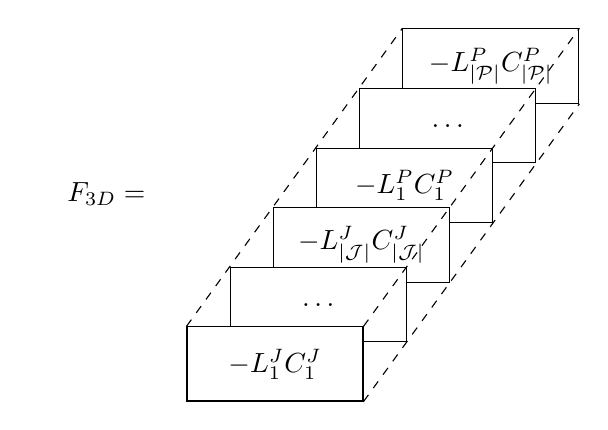
\begin{tikzpicture}[every node/.style={anchor=north east,fill=white,minimum width=2cm,minimum height=7mm}]
            
            % Define the displacement as a coordinate
            \coordinate (displacement) at (1.7,0.2);
        
            \matrix (mLCP) [draw,matrix of math nodes]
                {
                -L_{\cP}^PC_{\cP}^P \\
                };
        
            \matrix (dots2) [draw,matrix of math nodes] at ($(mLCP.south west)+(displacement)$)
                {
                \dots \\
                };
        
            \matrix (mLCp) [draw,matrix of math nodes] at ($(dots2.south west)+(displacement)$)
                {
                -L_{1}^PC_{1}^P \\
                };
        
            \matrix (mLCJ) [draw,matrix of math nodes] at ($(mLCp.south west)+(displacement)$)
                {
                -L_{\cJ}^JC_{\cJ}^J \\
                };
        
            \matrix (dots1) [draw,matrix of math nodes] at ($(mLCJ.south west)+(displacement)$)
                {
                \dots \\
                };
        
            \matrix (mLCj) [draw,matrix of math nodes] at ($(dots1.south west)+(displacement)$)
                {
                -L_1^JC_1^J \\
                };
            
            
            \draw[dashed](mLCj.north east)--(mLCP.north east);
            \draw[dashed](mLCj.north west)--(mLCP.north west);
            \draw[dashed](mLCj.south east)--(mLCP.south east);
            
            \node at ($(-5,-1.75)$) {$F_{3D}=$};
            
            \end{tikzpicture}
        \end{equation}
    \end{minipage}
\end{center}
and
\begin{center}
    \begin{minipage}[t]{0.4\textwidth}
        \centering
        % Second tikzpicture
        \begin{equation}\label{eqn:L-3d}
            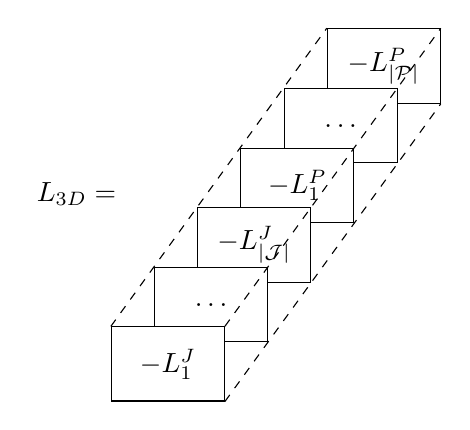
\begin{tikzpicture}[every node/.style={anchor=north east,fill=white,minimum width=1.2cm,minimum height=7mm}]
            
            % Define the displacement as a coordinate
            \coordinate (displacement) at (0.9,0.2);
        
            \matrix (mLP) [draw,matrix of math nodes]
                {
                -L_{\cP}^P \\
                };
        
            \matrix (dots2) [draw,matrix of math nodes] at ($(mLP.south west)+(displacement)$)
                {
                \dots \\
                };
        
            \matrix (mLp) [draw,matrix of math nodes] at ($(dots2.south west)+(displacement)$)
                {
                -L_{1}^P \\
                };
        
            \matrix (mLJ) [draw,matrix of math nodes] at ($(mLp.south west)+(displacement)$)
                {
                -L_{\cJ}^J \\
                };
        
            \matrix (dots1) [draw,matrix of math nodes] at ($(mLJ.south west)+(displacement)$)
                {
                \dots \\
                };
        
            \matrix (mLj) [draw,matrix of math nodes] at ($(dots1.south west)+(displacement)$)
                {
                -L_1^J \\
                };
            
            \draw[dashed](mLj.north east)--(mLP.north east);
            \draw[dashed](mLj.north west)--(mLP.north west);
            \draw[dashed](mLj.south east)--(mLP.south east);
            
            \node at ($(-4,-1.75)$) {$L_{3D}=$};
            
            \end{tikzpicture}
        \end{equation}
    \end{minipage}
    \begin{minipage}[t]{0.4\textwidth}
    \centering
    % Second tikzpicture
        \begin{equation}\label{eqn:eta-3d}
            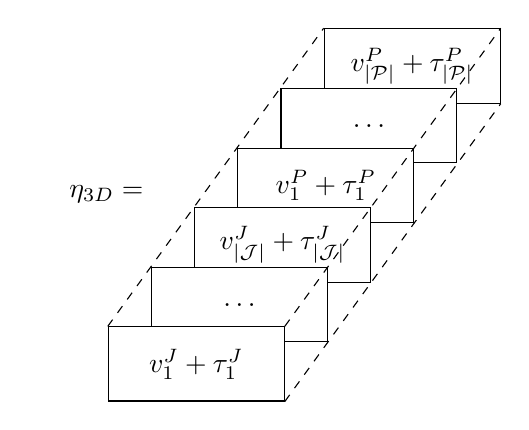
\begin{tikzpicture}[every node/.style={anchor=north east,fill=white,minimum width=2cm,minimum height=7mm}]
            
            % Define the displacement as a coordinate
            \coordinate (displacement) at (1.7,0.2);
        
            \matrix (mLP) [draw,matrix of math nodes]
                {
                v_{\cP}^P + \tau_{\cP}^P \\
                };
        
            \matrix (dots2) [draw,matrix of math nodes] at ($(mLP.south west)+(displacement)$)
                {
                \dots \\
                };
        
            \matrix (mLp) [draw,matrix of math nodes] at ($(dots2.south west)+(displacement)$)
                {
                v_1^P + \tau_1^P \\
                };
        
            \matrix (mLJ) [draw,matrix of math nodes] at ($(mLp.south west)+(displacement)$)
                {
                v_{\cJ}^J + \tau_{\cJ}^J \\
                };
        
            \matrix (dots1) [draw,matrix of math nodes] at ($(mLJ.south west)+(displacement)$)
                {
                \dots \\
                };
        
            \matrix (mLj) [draw,matrix of math nodes] at ($(dots1.south west)+(displacement)$)
                {
                v_1^J + \tau_1^J \\
                };
            
            \draw[dashed](mLj.north east)--(mLP.north east);
            \draw[dashed](mLj.north west)--(mLP.north west);
            \draw[dashed](mLj.south east)--(mLP.south east);
            
            \node at ($(-4,-1.75)$) {$\eta_{3D}=$};
            
            \end{tikzpicture}
        \end{equation}
    \end{minipage}
\end{center}

We can now construct all observers \eqref{eqn:cmo-single-J-observer}\eqref{eqn:cmo-single-P-observer} with the 3D matrices \eqref{eqn:x3d}\eqref{eqn:A-tilde-3D}\eqref{eqn:F-3d}\eqref{eqn:L-3d}\eqref{eqn:eta-3d}

\begin{equation*}
    \dot{\tilde{x}}_{3D} = \pamu(\tilde{A}_{3D},\tilde{x}_{3D},3) + \pamu(F_{3D},x,3) + \pamu(L_{3D},\eta_{3D},3) + \texttt{rep}(Bu + E\phi(y),N_S).
\end{equation*}

Let us now look at the sizes of all matrices that are required for state estimation. The matrices $L_{3D}$ and $\eta_{3D}$ are not taken into account, since they are only used to model the state estimators and would not be required in a physical implementation.
\begin{table}[h]
    \centering
    \begin{tabular}{c|c|c}
       Matrix  & Dimensions & Number of elements \\ \hline
       $\Tilde{x}_{3D}$  & $ n \times 1 \times N_S$ & $nN_S$ \\
       $\Tilde{A}_{3D}$ & $n \times n \times N_S$ & $n^2N_S$ \\ 
       $F_{3D}$ & $n \times n \times N_S$ & $n^2N_S$ \\
       
    \end{tabular}
    \caption{3D-CMO system matrix dimensions}
    \label{tab:3D-CMO-dimensions}
\end{table}


\subsection{Number of observers}
Let us define
\begin{equation}
    N_S = N_J + N_P
\end{equation}
which is the total number of systems needed for this multi-observer.\\

From the combinatoric nature of equation \eqref{eqn:multi-observer-sizes} it can be seen that the number of observers required to provide the secure state-estimate grows rapidly with the number of outputs $N$. Let us look more closely at $\cJ$ when $M$ is the largest integer so that $N>2M$ holds and thus equation \eqref{eqn:multi-observer-sizes} holds.
\begin{equation*}
    \begin{split}
        N_J &= {N_O \choose N_O-N_M}  = \frac{N_O!}{(N_O-M)!N_M!} = {N_O \choose N_M} \\
    \end{split}
\end{equation*}
which follows from the symmetry property of a combination \cite[Section 1.1]{Mazur2010PrinciplesCombinatorics}. Substituting this into $N_S$ results in
\begin{equation*}
    N_S = \frac{N_O!}{(N_O-N_M)!N_M!} + N_O,
\end{equation*}
which can be simplified into
\begin{equation*}
    N_S \approx \frac{N_O!}{(N_O-M)!N_M!}
\end{equation*}
for large $N_O$, when the combinatoric term dominates. Let us assume that $N_M=\frac{1}{2}N$ and substitute it in
\begin{equation}\label{eqn:simplified-NS}
    N_S \approx \frac{N_O!}{(N_O-\frac{1}{2}N_O)!(\frac{1}{2}N_O)!} = \frac{N_O!}{\left( \left( \frac{1}{2}N_O \right) ! \right)^2}.
\end{equation}
This requires taking a factorial of a non-integer, which is not defined. We therefore use \textit{Stirling's formula}\cite{Beals2012GammaZeta}, which states that
\begin{equation}\label{eqn:stirlings-formula}
    n! \sim \sqrt{2\pi n} \left( \frac{n}{e} \right)^n,
\end{equation}
where the $\sim$ implies that the ratio between the two sides of the equation approaches $1$ as $N_O \rightarrow \infty$. Let us now substitute \eqref{eqn:stirlings-formula} into \eqref{eqn:simplified-NS}
\begin{equation*}
    \begin{split}
        N_S \approx  \frac{\sqrt{2 \pi N_O}( \frac{N_O}{e} )^{N_O}}{\left( \sqrt{\pi N_O}(\frac{1}{2} \frac{N_O}{e} )^{\frac{1}{2}N_O} \right)^2} &= \frac{\sqrt{2 \pi N_O}}{\pi N_O} \frac{( \frac{N_O}{e} )^{N_O}}{(\frac{1}{2} \frac{N_O}{e} )^{N_O}} = \sqrt{\frac{2}{\pi N_O}} \frac{( \frac{N_O}{e} )^{N_O}}{(\frac{1}{2})^{N_O} (\frac{N_O}{e} )^{N_O}} \\
    \end{split}
\end{equation*}
which can be further simplified into
\begin{equation}\label{eqn:NS-approximation}
    N_S \approx \sqrt{\frac{2}{\pi N_O}}2^{N_O}.
\end{equation}
We now have an estimate that will be used to compare the sizes of different MO implementations.
\newpage
\section{Conventional multi-observer}\label{ch:cmo}
In this section the CMO will be introduced and two implementations will be discussed. Let us first further elaborate on the what the CMO should achieve. Let us look at the case where a 'single'-observer \eqref{eqn:unstable-simple-state-estimator} is employed to construct the state estimate of system \eqref{eqn:standard-system}, where $w=0$ and $v=0$. When an attacker gains control over some of the outputs $y_i$ and attacks it with the attack signal $\tau_i$. Performing the same analysis on the derivative of error \eqref{eqn:estimate-error} leads to
\begin{equation*}
    \begin{split}
        \dot{e} = \dot{\hat{x}} - \dot{x} &= A\hat{x} + Bu + E\phi(y) + L(C\hat{x} - Cx - \tau) - Ax - Bu - E\phi(y) \\
        &= (A+LC)e - L\tau,
    \end{split}
\end{equation*}
which does not guarantee $e \rightarrow 0$ as $t \rightarrow \infty$. The CMO aims to still provide a correct state estimate even when a subset $\mathcal{M} \subset \mathcal{N}$ outputs are under attack, where $2|\mathcal{M}| < |\mathcal{N}|$. 

\subsection{Constructing the state estimates}
\label{subsec:state-estimates}
The multi-observer described in this section is based on \cite[III B]{Chong2015ObservabilityAttacks}. This CMO is able to correctly estimate the state when up to $N_M = |\mathcal{M}|$ outputs are under attack. $N_M$ is required to satisfy $2N_M<N_O$, in other words: more than half the sensors need to remain attack free at all times. Consider system \eqref{eqn:standard-system} with $N_O$ outputs
\begin{equation*}
    \begin{split}
    \dot{x} &= Ax + Bu + E\phi(y) + w \\
        y_i &= C_ix + Du + v_i + \tau_i \quad i  \in \{1,2,\dots,N_O\}.
    \end{split}
\end{equation*}
Let us define $\mathcal{J} \subset \{1,2,\dots,N\}$ and $\mathcal{P} \subset \{1,2,\dots,N\}$ as all sets with  $J=N_O-N_M$ and  $P=1$ elements respectively. $P$ could also be taken as any value smaller than $J$, we restrict ourselves to systems that are fully observable trough any single output $y_i = C_ix$. The cardinalities of $\mathcal{J}$ and $\mathcal{P}$ are 
\begin{equation}\label{eqn:multi-observer-sizes}
    N_J = \cJ={N_O \choose J}={N_O \choose N_O-N_M}, \quad N_P = \cP = {N_O \choose P} = N_O.
\end{equation}
For example, $N_O=17$ and $N_M=8$ ($N_O>2N_M$) leads to $N_J=24310$ and $N_P=17$.
We now define the $j=1,2,\dots,N_J$ $J$\textit{-observers} as
\begin{equation*}
    \begin{split}
        \dot{\hat{x}}_j^\mcJ &= A\hat{x}_j^\mcJ + Bu + E\phi(y) + L_j(\hat{y}_j^\mcJ - y_j) \\
        \hat{y}_j^\mcJ &= C_j\hat{x}_j^\mcJ + Du
    \end{split}
\end{equation*}
where $j$ is a single combination out of all outputs and $L_j$ is an output injection gain that can be chosen in such a way to place the eigenvalues at a desired location if and only if the pair $(A,C_j)$ is observable. For example when $N_O=5$ and $N_M=2$, a possible $j$ is $\{1,3,4\}$ or $\{2,3,5\}$. The $J$ in the superscript indicates that this is a variable that relates to an observer that uses $J$ out of $N_O$ outputs.
Substituting $\hat{y}_j^J$ and $y_j$ in $\dot{\hat{x}}_j^J$ leads to
\begin{equation}\label{eqn:cmo-single-J-observer}
    \begin{split}
        \dot{\hat{x}}_j^{\mcJ} &= Ax_j^{\mcJ} + Bu + E\phi(y) + L_j^{\mcJ}(C\hat{x}_j^{\mcJ} + Du - C_j^{\mcJ}x - Du - v_j^{\mcJ}) \\
        \dot{\hat{x}}_j^{\mcJ} &= (A + L_j^{\mcJ}C_j^{\mcJ})\hat{x}_j - L_j^JC_j^{\mcJ}x + Bu + E\phi(y) - L_j^{\mcJ}(v_j^{\mcJ} + \tau_j^{\mcJ}). \\
    \end{split}    
\end{equation}
Doing the same for the the $p=1,2,\dots,N_P$ $P$\textit{-observers} leads to
\begin{equation}\label{eqn:cmo-single-P-observer}
    \dot{\hat{x}}_p^{\mcP} = (A + L_p^{\mcP}C_p^{\mcP})\hat{x}_p^{\mcP} - L_p^{\mcP}C_p^{\mcP}x + Bu + E\phi(y) - L_p^{\mcP}(v_p^{\mcP} + \tau_p^{\mcP}).
\end{equation}
Where $C_p$ and $C_i$ are the rows. All observers in \eqref{eqn:cmo-single-J-observer} and \eqref{eqn:cmo-single-P-observer} form a \textit{multi-observer}. Note that for a system with $N_M$ the largest possible number so that $N_O > 2N_M$, there is exactly one possible combination with $J$ elements out of all $N_J$ possible combinations that does not contain any of the $N_M$ attacked outputs. We now need to derive a method to select this one attack free observer from all observers. That is where the $P$-observers are used.

\subsection{Final estimate selection procedure}
\label{subsec:estimate-selection}
Now that all state estimates are constructed, a 'final' estimate $\hat{x}$ needs to be selected from all $\hat{x}_j^{\mcJ}$ First, a comparison will be made between all $J$-observers and the $P$-observers that are \textit{sub-observers}, implying that all outputs used to construct the state estimate $\hat{x}_p^{\mcP}$ are also used in the state estimate $\hat{x}_j^{\mcJ}$. For example, when $N_O=4$ $N_M=1$ one of the $J$-observer uses $j=\{1,2,4\}$ as outputs. The $P$-estimates would be constructed with $p \in \{1,2,4\}$. Let us define 
\begin{equation*}
   \pi_{j} = \max_{p \subset j} |\hat{x}_{j} - \hat{x}_{p}|
\end{equation*}
so the largest difference between the $j$-estimate and its $p$-estimates, where the $p$-observers are all a sub-observers of the $j$-observer. We now collect all $\pi_j$ in
\begin{equation*}
   \pi_{\mathcal{J}} = \max_{\mathcal{P} \subset \mathcal{J}} |\hat{x}_{\mathcal{J}} - \hat{x}_{\mathcal{P}}|
\end{equation*}

where $\hat{x}_{\mathcal{J}}$ are all state estimates from \eqref{eqn:cmo-single-J-observer} and $\hat{x}_{\mathcal{P}}$ are all sub-observers off each $j \in \mcJ$. Let us now choose the smallest $\pi_J$
\begin{equation}
    \sigma = \arg \min \pi_{\mathcal{J}}, \quad \sigma \subset \{1,2,\dots,N_J\}.
\end{equation}
We can now select the final state estimate as
\begin{equation}
    \hat{x} = \hat{x}_{\sigma}.
\end{equation}
This selection procedure selects the observer which has the smallest difference between itself and its sub-observers. 

\subsection{Observer architecture}
The state estimates constructed in \ref{subsec:state-estimates} only serve as a basis of the CMO, in this subsection two different implementations will be discussed. These implementations will be implemented in Matlab in the next chapter \textcolor{red}{ref this shit}. The first one  stores all the observers in a 2D matrix and will thus be known as the 2D-CMO. The second implementation stores the observers in a 3D matrix and will thus be known as the 3D-CMO.

\subsubsection{2D conventional multi-observer}
\textcolor{red}{decide if I want to keep this in, would require fintuning the implementation and adding the nonlinearity}
Let us write all observers \eqref{eqn:cmo-single-J-observer}\eqref{eqn:cmo-single-P-observer} in the following form
\begin{equation*}
    \dot{\Tilde{x}}_{2D} = \Tilde{A}_{2D}\Tilde{x}_{2D} + F_{2D}\eta_{2D}
\end{equation*}
where
\begin{equation}\label{eqn:2D-CMO}
\renewcommand{\arraystretch}{1.3}
    \begin{split}    
        \Tilde{x}_{2D} &= 
        \begin{bmatrix}
            \hat{x}_1^{\mcJ} \\ \vdots \\ \hat{x}_{N_J}^{\mcJ} \\ \hat{x}_1^{P} \\ \vdots \\ \hat{x}_{N_P}^{\mcP}
        \end{bmatrix}, \quad
        \Tilde{A}_{2D} = 
        \begin{bmatrix}
            -L_1^{\mcJ}C_1^{\mcJ} & A + L_1^{\mcJ}C_1^{\mcJ} & \cdots & 0  & 0 & \cdots & 0 \\
            \vdots & \vdots & \ddots & \vdots & \vdots & & \vdots \\
            -L_{N_J}^{\mcJ}C_{N_J}^{\mcJ} & 0 & \cdots & A + L_{N_J}^{\mcJ}C_{N_J}^{\mcJ} & 0 & \cdots & 0 \\
            -L_{1}^{\mcP}C_{1}^{\mcP} & 0 & \cdots & 0 & A + L_1^{\mcP}C_1^{\mcP} & \cdots & 0 \\
            \vdots & \vdots &  & \vdots & \vdots & \ddots & \vdots \\
            -L_{N_P}^{\mcP}C_{N_P}^{\mcP} & 0 & \cdots & 0 & 0 & \cdots & A + L_{N_P}^{\mcP}C_{N_P}^{\mcP} \\
        \end{bmatrix} \\
        \eta &= 
        \begin{bmatrix}
            u \\ v_1^{\mcJ} + \tau_1^{\mcJ} \\ \vdots \\ v_{N_J}^{\mcJ} + \tau_{N_J}^J \\ v_1^{\mcP} + \tau_1^{\mcP} \\ \vdots \\ v_{N_P}^{\mcP} + \tau_{N_P}^{\mcP} \\ w \\
        \end{bmatrix}, \quad 
        F_{2D} = 
        \begin{bmatrix}
            B & -L_1^{\mcJ} & \cdots & 0 & 0 & \cdots & 0 \\
            \vdots & \vdots & \ddots & \vdots & \vdots & & \vdots \\
            B & 0 & \cdots & -L_{\cJ}^{\mcJ} & 0 & \cdots & 0 \\
            B & 0 & \cdots & 0 & -L_{1}^{\mcP} & \cdots & 0 \\
            \vdots & \vdots & & \vdots & \vdots & \ddots & \vdots \\
            B & 0 & \cdots & 0 & 0 & \cdots & -L_{N_P}^{\mcP} \\
        \end{bmatrix}\\
    \end{split}
\end{equation}
The $\Tilde{A}$ matrix stores  all $J$- and $P$-estimates: the top section stores the $J$-observers and on the bottom the $P$-observers. Multiplying this $\Tilde{A}_{2D}$ matrix by $\Tilde{x}_{2D}$ leads to the state estimators presented in \eqref{eqn:cmo-single-J-observer} and \eqref{eqn:cmo-single-P-observer} without inputs, noise and attacks. The vector $\eta$ stacks the input and sum of sensor noise and attack signal on top of each other and the matrix $E$ stores all factors that need to be multiplied with $\eta$ to arrive at \eqref{eqn:cmo-single-J-observer} and \eqref{eqn:cmo-single-P-observer}.

\begin{table}[h]
    \centering
    \begin{tabular}{c|c|c}
       Matrix  & Dimensions & Number of elements \\ \hline
       $\Tilde{x}_{2D}$  & $n_xN_S \times 1$ & $n_xN_S$ \\
       $\Tilde{A}_{2D}$ & $n_xN_S \times n_xN_S$ & $n_x^2N_S^2$ \\
       $B_{2D}$ & $n_u \times N_S$ & $n_uN_S$ \\
       $u_{2D}$ & $n_u \times N_S$ & $n_uN_S$ \\
    \end{tabular}
    \caption{2D-CMO system matrix dimensions}
    \label{tab:2D-CMO-dimensions}
\end{table}



\newpage
\subsubsection{3D conventional multi-observer}
Now the second implementation of the CMO will be discussed. The goal of the 3D-CMO is to reduce the number of zeros required in the $\Tilde{A}_{2D}$\eqref{eqn:2D-CMO}. In order to do so we store all block matrices behind each other. Let us start by defining 
\begin{center}
    \begin{minipage}[t]{0.4\textwidth}
        \centering
        % First tikzpicture
        \begin{equation}\label{eqn:x3d}
            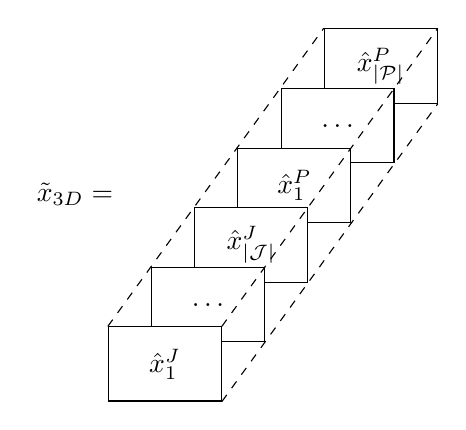
\begin{tikzpicture}[every node/.style={anchor=north east,fill=white,minimum width=1.2cm,minimum height=7mm}] 
            % Define the displacement as a coordinate
            \coordinate (displacement) at (0.9,0.2);
        
            \matrix (mxP) [draw,matrix of math nodes]
                {
                \hat{x}_{\cP}^P \\
                };
        
            \matrix (dots2) [draw,matrix of math nodes] at ($(mxP.south west)+(displacement)$)
                {
                \dots \\
                };
        
            \matrix (mxp) [draw,matrix of math nodes] at ($(dots2.south west)+(displacement)$)
                {
                \hat{x}_1^P \\
                };
        
            \matrix (mxJ) [draw,matrix of math nodes] at ($(mxp.south west)+(displacement)$)
                {
                \hat{x}_{\cJ}^J \\
                };
        
            \matrix (dots1) [draw,matrix of math nodes] at ($(mxJ.south west)+(displacement)$)
                {
                \dots \\
                };
        
            \matrix (mxj) [draw,matrix of math nodes] at ($(dots1.south west)+(displacement)$)
                {
                \hat{x}_1^J \\
                };
    
            \node at ($(-4,-1.75)$) {$\tilde{x}_{3D}=$};
            
            \draw[dashed](mxj.north east)--(mxP.north east);
            \draw[dashed](mxj.north west)--(mxP.north west);
            \draw[dashed](mxj.south east)--(mxP.south east);
    
        \end{tikzpicture}
        \end{equation}
    \end{minipage}
    \begin{minipage}[t]{0.4\textwidth}
        \centering
        % Second tikzpicture
        \begin{equation}\label{eqn:A-tilde-3D}
            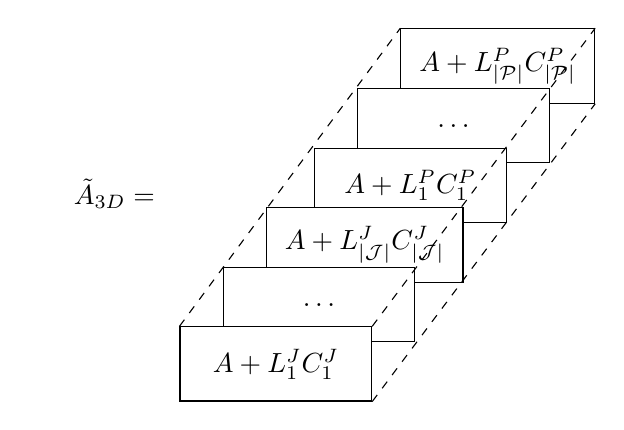
\begin{tikzpicture}[every node/.style={anchor=north east,fill=white,minimum width=2.2cm,minimum height=7mm}]
            
            % Define the displacement as a coordinate
            \coordinate (displacement) at (1.9,0.2);
        
            \matrix (mAP) [draw,matrix of math nodes]
                {
                A + L_{\cP}^PC_{\cP}^P \\
                };
        
            \matrix (dots2) [draw,matrix of math nodes] at ($(mAP.south west)+(displacement)$)
                {
                \dots \\
                };
        
            \matrix (mAp) [draw,matrix of math nodes] at ($(dots2.south west)+(displacement)$)
                {
                A + L_1^PC_1^P \\
                };
        
            \matrix (mAJ) [draw,matrix of math nodes] at ($(mAp.south west)+(displacement)$)
                {
                A + L_{\cJ}^JC_{\cJ}^J \\
                };
        
            \matrix (dots1) [draw,matrix of math nodes] at ($(mAJ.south west)+(displacement)$)
                {
                \dots \\
                };
        
            \matrix (mAj) [draw,matrix of math nodes] at ($(dots1.south west)+(displacement)$)
                {
                A + L_1^J C_1^J \\
                };
            
            \draw[dashed](mAj.north east)--(mAP.north east);
            \draw[dashed](mAj.north west)--(mAP.north west);
            \draw[dashed](mAj.south east)--(mAP.south east);
        
            \node at ($(-5,-1.75)$) {$\tilde{A}_{3D}=$};
            
            \end{tikzpicture}
        \end{equation}
    \end{minipage}
\end{center}

$\tilde{x}_{3D}$ is similar to $\tilde{x}_{2D}$ \eqref{eqn:2D-CMO}, where the state $x$ and all its state estimates are stored below each other. Let us now define some basic notation, similar to Matlab notation, regarding three-dimensional arrays. We will define a \textit{page} of a 3D array as a single 2D slice from that array, these slices can be taken from any 2 dimensions present in the 3D array. Let us define $G \in \mathbb{R}^{3 \times 4 \times 8}$, slicing the first page along the third dimension will be denoted as $G(:,:,1)$ and the third page along the first dimension as $G(3,:,:)$. The slices that can be seen in equation \eqref{eqn:A-tilde-3D} are sliced along the third dimension. \\
$\tilde{A}_{3D}$ stores all elements on the diagonal of $\tilde{A}_{2D}$ \eqref{eqn:2D-CMO} on a separate page of a 3D array. Let us now define the operation \textit{page multiplication}, this operation can be performed on two 3D arrays that have (at least) one equal dimension and pages sliced along this equal dimension result in two matrices that can be multiplied. Or one 3D matrix and a 2D matrix where slicing the 3D matrix along the desired dimension results in slices that can be multiplied with the 2D matrix. This operation is analogous with the Matlab function \texttt{pagemtimes} \cite{2022MATLABR2022b}. In this report a page multiplication of two  matrices $A$ and $B$ along the third dimension will be denoted as $ \pamu(A,B,3)$. \\
Another operation is required for the summands that are equal for each observer, $Bu$ and $E\phi(y)$. The multiplication only has to be performed once and the resultant matrix $M$ should be repeated along the third dimension $n$ times. This operation is analogous to the Matlab function \texttt{repmat}(M,1,1,n) \cite{2022MATLABR2022b}. In this report this function will be denoted as \texttt{rep}(M,n), where the ones indicating the number of repetitions are omitted. Let us now define

\begin{center}
    \begin{minipage}[t]{0.4\textwidth}
        % First tikzpicture
        \begin{equation}\label{eqn:F-3d}
            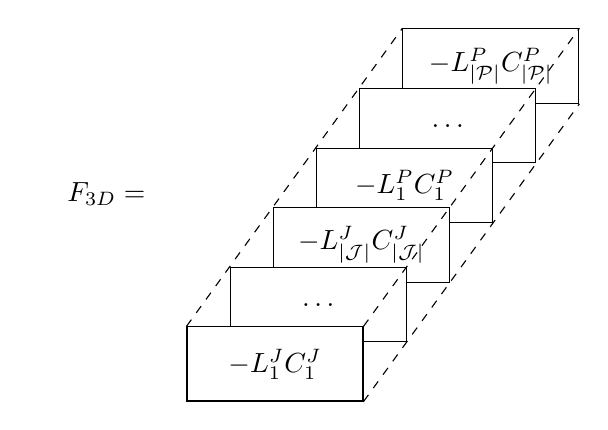
\begin{tikzpicture}[every node/.style={anchor=north east,fill=white,minimum width=2cm,minimum height=7mm}]
            
            % Define the displacement as a coordinate
            \coordinate (displacement) at (1.7,0.2);
        
            \matrix (mLCP) [draw,matrix of math nodes]
                {
                -L_{\cP}^PC_{\cP}^P \\
                };
        
            \matrix (dots2) [draw,matrix of math nodes] at ($(mLCP.south west)+(displacement)$)
                {
                \dots \\
                };
        
            \matrix (mLCp) [draw,matrix of math nodes] at ($(dots2.south west)+(displacement)$)
                {
                -L_{1}^PC_{1}^P \\
                };
        
            \matrix (mLCJ) [draw,matrix of math nodes] at ($(mLCp.south west)+(displacement)$)
                {
                -L_{\cJ}^JC_{\cJ}^J \\
                };
        
            \matrix (dots1) [draw,matrix of math nodes] at ($(mLCJ.south west)+(displacement)$)
                {
                \dots \\
                };
        
            \matrix (mLCj) [draw,matrix of math nodes] at ($(dots1.south west)+(displacement)$)
                {
                -L_1^JC_1^J \\
                };
            
            
            \draw[dashed](mLCj.north east)--(mLCP.north east);
            \draw[dashed](mLCj.north west)--(mLCP.north west);
            \draw[dashed](mLCj.south east)--(mLCP.south east);
            
            \node at ($(-5,-1.75)$) {$F_{3D}=$};
            
            \end{tikzpicture}
        \end{equation}
    \end{minipage}
\end{center}
and
\begin{center}
    \begin{minipage}[t]{0.4\textwidth}
        \centering
        % Second tikzpicture
        \begin{equation}\label{eqn:L-3d}
            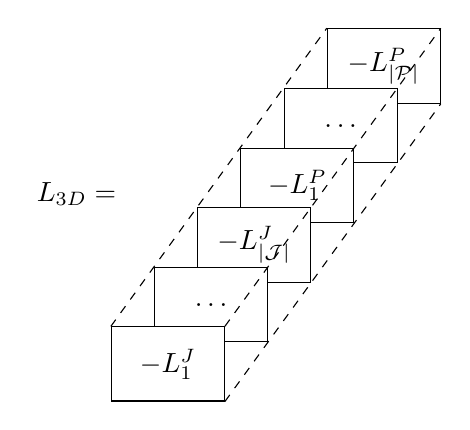
\begin{tikzpicture}[every node/.style={anchor=north east,fill=white,minimum width=1.2cm,minimum height=7mm}]
            
            % Define the displacement as a coordinate
            \coordinate (displacement) at (0.9,0.2);
        
            \matrix (mLP) [draw,matrix of math nodes]
                {
                -L_{\cP}^P \\
                };
        
            \matrix (dots2) [draw,matrix of math nodes] at ($(mLP.south west)+(displacement)$)
                {
                \dots \\
                };
        
            \matrix (mLp) [draw,matrix of math nodes] at ($(dots2.south west)+(displacement)$)
                {
                -L_{1}^P \\
                };
        
            \matrix (mLJ) [draw,matrix of math nodes] at ($(mLp.south west)+(displacement)$)
                {
                -L_{\cJ}^J \\
                };
        
            \matrix (dots1) [draw,matrix of math nodes] at ($(mLJ.south west)+(displacement)$)
                {
                \dots \\
                };
        
            \matrix (mLj) [draw,matrix of math nodes] at ($(dots1.south west)+(displacement)$)
                {
                -L_1^J \\
                };
            
            \draw[dashed](mLj.north east)--(mLP.north east);
            \draw[dashed](mLj.north west)--(mLP.north west);
            \draw[dashed](mLj.south east)--(mLP.south east);
            
            \node at ($(-4,-1.75)$) {$L_{3D}=$};
            
            \end{tikzpicture}
        \end{equation}
    \end{minipage}
    \begin{minipage}[t]{0.4\textwidth}
    \centering
    % Second tikzpicture
        \begin{equation}\label{eqn:eta-3d}
            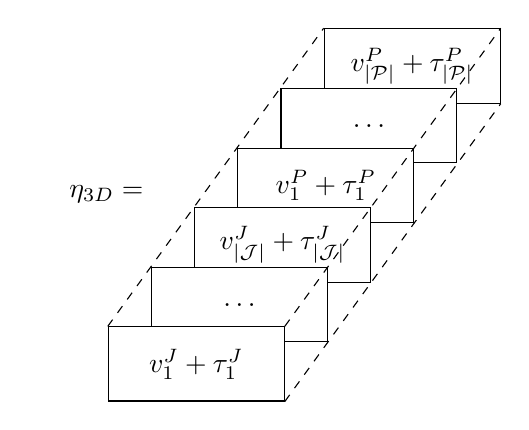
\begin{tikzpicture}[every node/.style={anchor=north east,fill=white,minimum width=2cm,minimum height=7mm}]
            
            % Define the displacement as a coordinate
            \coordinate (displacement) at (1.7,0.2);
        
            \matrix (mLP) [draw,matrix of math nodes]
                {
                v_{\cP}^P + \tau_{\cP}^P \\
                };
        
            \matrix (dots2) [draw,matrix of math nodes] at ($(mLP.south west)+(displacement)$)
                {
                \dots \\
                };
        
            \matrix (mLp) [draw,matrix of math nodes] at ($(dots2.south west)+(displacement)$)
                {
                v_1^P + \tau_1^P \\
                };
        
            \matrix (mLJ) [draw,matrix of math nodes] at ($(mLp.south west)+(displacement)$)
                {
                v_{\cJ}^J + \tau_{\cJ}^J \\
                };
        
            \matrix (dots1) [draw,matrix of math nodes] at ($(mLJ.south west)+(displacement)$)
                {
                \dots \\
                };
        
            \matrix (mLj) [draw,matrix of math nodes] at ($(dots1.south west)+(displacement)$)
                {
                v_1^J + \tau_1^J \\
                };
            
            \draw[dashed](mLj.north east)--(mLP.north east);
            \draw[dashed](mLj.north west)--(mLP.north west);
            \draw[dashed](mLj.south east)--(mLP.south east);
            
            \node at ($(-4,-1.75)$) {$\eta_{3D}=$};
            
            \end{tikzpicture}
        \end{equation}
    \end{minipage}
\end{center}

We can now construct all observers \eqref{eqn:cmo-single-J-observer}\eqref{eqn:cmo-single-P-observer} with the 3D matrices \eqref{eqn:x3d}\eqref{eqn:A-tilde-3D}\eqref{eqn:F-3d}\eqref{eqn:L-3d}\eqref{eqn:eta-3d}

\begin{equation*}
    \dot{\tilde{x}}_{3D} = \pamu(\tilde{A}_{3D},\tilde{x}_{3D},3) + \pamu(F_{3D},x,3) + \pamu(L_{3D},\eta_{3D},3) + \texttt{rep}(Bu + E\phi(y),N_S).
\end{equation*}

Let us now look at the sizes of all matrices that are required for state estimation. The matrices $L_{3D}$ and $\eta_{3D}$ are not taken into account, since they are only used to model the state estimators and would not be required in a physical implementation.
\begin{table}[h]
    \centering
    \begin{tabular}{c|c|c}
       Matrix  & Dimensions & Number of elements \\ \hline
       $\Tilde{x}_{3D}$  & $ n_x \times 1 \times N_S$ & $n_xN_S$ \\
       $\Tilde{A}_{3D}$ & $n_x \times n_x \times N_S$ & $n_x^2N_S$ \\ 
       $F_{3D}$ & $n_x \times n_x \times N_S$ & $n_x^2N_S$ \\
       
    \end{tabular}
    \caption{3D-CMO system matrix dimensions}
    \label{tab:3D-CMO-dimensions}
\end{table}


\subsection{Number of observers}
Let us define
\begin{equation}
    N_S = N_J + N_P
\end{equation}
which is the total number of systems needed for this multi-observer.\\

From the combinatoric nature of equation \eqref{eqn:multi-observer-sizes} it can be seen that the number of observers required to provide the secure state-estimate grows rapidly with the number of outputs $N$. Let us look more closely at $\cJ$ when $M$ is the largest integer so that $N>2M$ holds and thus equation \eqref{eqn:multi-observer-sizes} holds.
\begin{equation*}
    \begin{split}
        N_J &= {N_O \choose N_O-N_M}  = \frac{N_O!}{(N_O-M)!N_M!} = {N_O \choose N_M} \\
    \end{split}
\end{equation*}
which follows from the symmetry property of a combination \cite[Section 1.1]{Mazur2010PrinciplesCombinatorics}. Substituting this into $N_S$ results in
\begin{equation*}
    N_S = \frac{N_O!}{(N_O-N_M)!N_M!} + N_O,
\end{equation*}
which can be simplified into
\begin{equation*}
    N_S \approx \frac{N_O!}{(N_O-M)!N_M!}
\end{equation*}
for large $N_O$, when the combinatoric term dominates. Let us assume that $N_M=\frac{1}{2}N$ and substitute it in
\begin{equation}\label{eqn:simplified-NS}
    N_S \approx \frac{N_O!}{(N_O-\frac{1}{2}N_O)!(\frac{1}{2}N_O)!} = \frac{N_O!}{\left( \left( \frac{1}{2}N_O \right) ! \right)^2}.
\end{equation}
This requires taking a factorial of a non-integer, which is not defined. We therefore use \textit{Stirling's formula}\cite{Beals2012GammaZeta}, which states that
\begin{equation}\label{eqn:stirlings-formula}
    n! \sim \sqrt{2\pi n} \left( \frac{n}{e} \right)^n,
\end{equation}
where the $\sim$ implies that the ratio between the two sides of the equation approaches $1$ as $N_O \rightarrow \infty$. Let us now substitute \eqref{eqn:stirlings-formula} into \eqref{eqn:simplified-NS}
\begin{equation*}
    \begin{split}
        N_S \approx  \frac{\sqrt{2 \pi N_O}( \frac{N_O}{e} )^{N_O}}{\left( \sqrt{\pi N_O}(\frac{1}{2} \frac{N_O}{e} )^{\frac{1}{2}N_O} \right)^2} &= \frac{\sqrt{2 \pi N_O}}{\pi N_O} \frac{( \frac{N_O}{e} )^{N_O}}{(\frac{1}{2} \frac{N_O}{e} )^{N_O}} = \sqrt{\frac{2}{\pi N_O}} \frac{( \frac{N_O}{e} )^{N_O}}{(\frac{1}{2})^{N_O} (\frac{N_O}{e} )^{N_O}} \\
    \end{split}
\end{equation*}
which can be further simplified into
\begin{equation}\label{eqn:NS-approximation}
    N_S \approx \sqrt{\frac{2}{\pi N_O}}2^{N_O}
\end{equation}
\newpage


\section{State-sharing multi-observer}
In this chapter the state-sharing multi-observer (SSMO) will be discussed, aiming to reduce the required memory to store the CMO. The SSMO described in this chapter will provide the estimates as described in \autoref{subsec:state-estimates} and will employ the same selection procedure as described in \autoref{subsec:estimate-selection}.

\subsection{Constructing the state-estimates}
Let
\begin{equation}\label{eqn:ssmo-observer}
    \begin{split}
        \dot{\hat{x}}_o &= \A_o\hat{x}_o - L_oC_ox + Bu -L_o(v_o + \tau_o), \quad \A_o=A+L_{o}C_{o} \\
    \end{split}
\end{equation}
be a set of observers that contains all $J$- and $P$-observers \eqref{eqn:cmo-single-J-observer}\eqref{eqn:cmo-single-P-observer}, such that $\mcO=\mcJ\bigcup\mcP$ and $o=1,2,\dots,|\mcO|$. All $L_o$ must be selected in such a way that all $\A_o$ share the same characteristic polynomial
\begin{equation}\label{eqn:ssmo-char-poly}
    \det(sI-\A) = p(s) = s^n + q_1s^{n-1} + \dots + q_{n-1}s + q_n
\end{equation}
and thus all have equal eigenvalues. Let us now define a matrix $\Tilde{L}_{o}$ such that $\Tilde{L}_oy=L_oy_o$. This can be achieved by padding $L_o$ with zero vectors $z \in \mathbb{R}^{n \times 1}$ \cite{Chong2023MemoryAlgorithms}. Let us now rewrite the observer \eqref{eqn:ssmo-observer} into the following form
\begin{equation}\label{eqn:ssmo-standard-system-form}
    \dot{\hat{x}}_o = \A_o\hat{x}_o + \B_o\eta_o, \quad
    \B_o =
    \begin{bmatrix}
        E & B & -\Tilde{L}_o \\
    \end{bmatrix}, \quad \eta_o =
    \begin{bmatrix}
        \phi(y) \\
        u \\
        y_o + v_o + \tau_o
    \end{bmatrix}.
\end{equation}

Let us now derive transformation matrices $T_o$ that transform all $\A_o=A+L_{o}C_{o}$ into controllable canonical form as in \cite[Sec. 4.3.2]{Hespanha2018LinearTheory}
\begin{equation}\label{eqn:controllable-canonical-form}
    \mathbf{A} =
    \begin{bmatrix}
        -q_1I_l & -q_2I_l & \cdots & -q_{n-1}I_l & -q_nI_l \\
        I_l & 0_l & \cdots & 0_l & 0_l \\
        0_l & I_l & \cdots & 0_l & 0_l \\
        \vdots & \vdots & \ddots & \vdots & \vdots \\
        0_l & 0_l & \cdots & I_l & 0_l \\
    \end{bmatrix}, \quad
    \mathbf{B} = 
    \begin{bmatrix}
        I_l \\ 0_l \\ \vdots \\ 0_l \\ 0_l \\
    \end{bmatrix}
\end{equation}
where $l=N$. The transformation matrices for each observer are $T_o=R_pR_q$,
\begin{equation}
    \begin{split}
         R_p &=
        \begin{bmatrix}
            \B_o & \A_o\B_o & \A^{2}_o\B_o & \cdots & \A^{n-1}_o\B_o \\
        \end{bmatrix} \\
        R_q &=
        \begin{bmatrix}
            I_l & q_1I_l & q_2I_l & \cdots & q_{n-1}I_l \\
            0_l & I_l & q_1I_l & \cdots & q_{n-2}I_l \\
            \vdots & \ddots & \ddots & \ddots & \vdots \\
            0_l & \cdots & 0_l & I_l & q_1I_l \\
            0_l & \cdots & 0_l & 0_l & I_l \\
        \end{bmatrix}.
    \end{split}
\end{equation}
Let us now show that the following
\begin{equation}\label{eqn:A-transformation}
    \begin{split}
        T_o\mathbf{A} &= \A_oT_o \\
        R_pR_q\mathbf{A} &= \A_oR_pR_q \\
    \end{split}
\end{equation}
holds. Let us start by expanding
\begin{equation*}
    \begin{split}
        R_q\mathbf{A} &=  
        \begin{bmatrix}
            I_l & q_1I_l & q_2I_l & \cdots & q_{n-1}I_l \\
            0_l & I_l & q_1I_l & \cdots & q_{n-2}I_l \\
            \vdots & \ddots & \ddots & \ddots & \vdots \\
            0_l & \cdots & 0_l & I_l & q_1I_l \\
            0_l & \cdots & 0_l & 0_l & I_l \\
        \end{bmatrix}
        \begin{bmatrix}
            -q_1I_l & -q_2I_l & \cdots & -q_{n-1}I_l & -q_nI_l \\
            I_l & 0_l & \cdots & 0_l & 0_l \\
            0_l & I_l & \cdots & 0_l & 0_l \\
            \vdots & \vdots & \ddots & \vdots & \vdots \\
            0_l & 0_l & \cdots & I_l & 0_l \\
        \end{bmatrix} \\
        &= 
        \begin{bmatrix}
            0_l & 0_l & 0_l & \cdots & 0_l & 0_l & 0_l \\
            I_l & q_1I_l & q_2I_l & \cdots & q_{n-3}I_l & q_{n-2}I_l & 0_l \\ 
            0_l & I_l & q_1I_l & \cdots & q_{n-4}I_l & q_{n-3}I_l & 0_l \\ 
            \vdots & \vdots & \vdots & \ddots & \vdots & \vdots & \vdots \\
            0_l & 0_l & 0_l & \cdots & q_1I_l & q_2I_l & 0_l \\
            0_l & 0_l & 0_l & \cdots & I_l & q_1I_l & 0_l \\
            0_l & 0_l & 0_l & \cdots & 0_l & I_l & 0_l \\
        \end{bmatrix}.
    \end{split} 
\end{equation*}
We now premultiply this by $R_o$
\begin{equation*}
    \begin{split}
        R_pR_q\mathbf{A} &= 
        \begin{bmatrix}
            \B_o & \A_o\B_o & \A^{2}_o\B_o & \cdots & \A^{n-1}_o\B_o \\
        \end{bmatrix}
        \begin{bmatrix}
            0_l & 0_l & 0_l & \cdots & 0_l & 0_l \\
            I_l & q_1I_l & q_2I_l & \cdots & q_{n-2}I_l & 0_l \\ 
            0_l & I_l & q_1I_l & \cdots & q_{n-3}I_l & 0_l \\ 
            \vdots & \ddots & \ddots & \ddots & \vdots & \vdots \\
            0_l & 0_l & 0_l & \ddots & q_1I_l & 0_l \\
            0_l & 0_l & 0_l & \cdots & I_l & 0_l \\
        \end{bmatrix} \\
        &= 
        \begin{bmatrix}
            \A_o\B_o \\ q_1\A_o\B_o + \A^2_o\B_o \\ q_2\A_o\B_o + q_1\A^2_o\B_o + \A^3_o\B_o \\ \cdots \\ q_{n-2}\A_o\B_o + q_{n-3}\A^2_o\B_o + \cdots + q_1\A^{n-2}_o\B_o + \A^{n-1}_o\B_o \\ 0 \\      
        \end{bmatrix}^T
    \end{split}
\end{equation*}
Where by the Cayley-Hamilton theorem we can rewrite penultimate column as
\begin{equation*}
    \begin{bmatrix}
            \A_o\B_o \\ q_1\A_o\B_o + \A^2_o\B_o \\ q_2\A_o\B_o + q_1\A^2_o\B_o + \A^3_o\B_o \\ \vdots \\ -\A^n_o\B_o \\ 0 \\      
        \end{bmatrix}^T
\end{equation*}

We now expand
\begin{equation*}
    \begin{split}
        \A_oR_pR_q &= 
        \begin{bmatrix}
            \A_o\B_o & \A^2_o\B_o & \A^{3}_o\B_o & \cdots & \A^{n}_o\B_o \\
        \end{bmatrix}
        \begin{bmatrix}
            I_l & q_1I_l & q_2I_l & \cdots & q_{n-1}I_l \\
            0_l & I_l & q_1I_l & \cdots & q_{n-2}I_l \\
            \vdots & \ddots & \ddots & \ddots & \vdots \\
            0_l & \cdots & 0_l & I_l & q_1I_l \\
            0_l & \cdots & 0_l & 0_l & I_l \\
        \end{bmatrix} \\
        &=
        \begin{bmatrix}
            \A_o\B_o \\ 
            q_1\A_o\B_o + \A^2_o\B_o \\ 
            q_2\A_o\B_o + q_1\A^2\B_o + \A^3_o\B_o \\ \vdots \\ 
            q_{n-1}\A_o\B_o + q_{n-2}\A^2_o\B_o + \cdots + \A^{n-1}_o\B_o \\
            q_{n-1}\A_o\B_o + q_{n-2}\A^2_o\B_o + \cdots + \A^{n-1}_o\B_o + \A^n_o\B_o \\
        \end{bmatrix}^T,
    \end{split}
\end{equation*}
where the bottom two rows can be simplified by using the Cayley-Hamilton theorem
\begin{equation*}
    \begin{split}
        \A_oR_pR_q &= 
        \begin{bmatrix}
            \A_o\B_o \\ 
            q_1\A_o\B_o + \A^2_o\B_o \\ 
            q_2\A_o\B_o + q_1\A^2\B_o + \A^3_o\B_o \\ \vdots \\ 
            \A^{n}_o\B_o \\
            0 \\
        \end{bmatrix}^T,
    \end{split}
\end{equation*}
which is equal to $R_oR_q\A_o$. We can now conclude that the matrix $T_o=R_oR_q$ satisfies \eqref{eqn:A-transformation}. Now we will show the same for
\begin{equation}\label{eqn:B-transformation}
    \begin{split}
        T_o\mathbf{B} &= \B_o \\
        R_pR_q\mathbf{B} &= \B_o.
    \end{split}
\end{equation}
Let us expand
\begin{equation*}
    \begin{split}
        R_pR_q\mathbf{B} &=
        \begin{bmatrix}
            \B_o & \A_o\B_o & \A^{2}_o\B_o & \cdots & \A^{n-1}_o\B_o \\
        \end{bmatrix}
        \begin{bmatrix}
            I_l & q_1I_l & q_2I_l & \cdots & q_{n-1}I_l \\
            0_l & I_l & q_1I_l & \cdots & q_{n-2}I_l \\
            \vdots & \ddots & \ddots & \ddots & \vdots \\
            0_l & \cdots & 0_l & I_l & q_1I_l \\
            0_l & \cdots & 0_l & 0_l & I_l \\
        \end{bmatrix}
        \begin{bmatrix}
            I_l \\ 0_l \\ \vdots \\ 0_l \\ 0_l \\
        \end{bmatrix} \\
        &=
        \begin{bmatrix}
            \B_o & \A_o\B_o & \A^{2}_o\B_o & \cdots & \A^{n-1}_o\B_o \\
        \end{bmatrix}
        \begin{bmatrix}
            I_l \\ 0_l \\ \vdots \\ 0_l \\ 0_l \\
        \end{bmatrix} = \B_o \\
    \end{split}
\end{equation*}
which shows that \eqref{eqn:B-transformation} holds. It should be noted that $\mathbf{A}$ and $\mathbf{B}$ are independent of $o$ and since all observers \eqref{eqn:ssmo-observer} share the same characteristic polynomial \eqref{eqn:ssmo-char-poly}, $\mathbf{A}$ and $\mathbf{B}$ are the same for all observers. This means that only one copy of the matrices needs to be stored and all state estimates $\hat{x}$ from the transformation matrices.

\subsection{Implementation}
Let us set the initial conditions of all state estimates to be equal, we will choose $0$ for simplicity. When all initial conditions are zero $z$ will also be the same for all state estimates, 
\begin{equation*}
    \dot{z} = \mathbf{A}z + \mathbf{B}\eta, \quad \eta = 
    \begin{bmatrix}
        u \\ y + v + \tau
    \end{bmatrix}.
\end{equation*}
We then transform $z$ into the original state estimates by

\begin{equation*}
    \tilde{x}_{SSMO} = \texttt{pm}(T,z,3),
\end{equation*}
where
\begin{center}
    % \begin{minipage}[t]{0.4\textwidth}
    %     \centering
    %     % first tikzpicture
    %     \begin{equation*}
    %         \begin{tikzpicture}[every node/.style={anchor=north east,fill=white,minimum width=1.2cm,minimum height=7mm}]
            
    %         % Define the displacement as a coordinate
    %         \coordinate (displacement) at (0.9,0.2);
        
    %         \matrix (mLP) [draw,matrix of math nodes]
    %             {
    %             \hat{x}_{\cP}^\mcJ \\
    %             };
        
    %         \matrix (dots2) [draw,matrix of math nodes] at ($(mLP.south west)+(displacement)$)
    %             {
    %             \dots \\
    %             };
        
    %         \matrix (mLp) [draw,matrix of math nodes] at ($(dots2.south west)+(displacement)$)
    %             {
    %             \hat{x}_{1}^\mcP \\
    %             };
        
    %         \matrix (mLJ) [draw,matrix of math nodes] at ($(mLp.south west)+(displacement)$)
    %             {
    %             \hat{x}_{\cJ}^\mcJ \\
    %             };
        
    %         \matrix (dots1) [draw,matrix of math nodes] at ($(mLJ.south west)+(displacement)$)
    %             {
    %             \dots \\
    %             };
        
    %         \matrix (mLj) [draw,matrix of math nodes] at ($(dots1.south west)+(displacement)$)
    %             {
    %             \hat{x}_1^\mcJ \\
    %             };
            
    %         \draw[dashed](mLj.north east)--(mLP.north east);
    %         \draw[dashed](mLj.north west)--(mLP.north west);
    %         \draw[dashed](mLj.south east)--(mLP.south east);
            
    %         \node at ($(-4,-1.8)$) {$\hat{x}_{SSMO}=$};
            
    %         \end{tikzpicture}
    %     \end{equation*}
    % \end{minipage}
    \begin{minipage}[t]{0.4\textwidth}
    \centering
    % Second tikzpicture
        \begin{equation}
            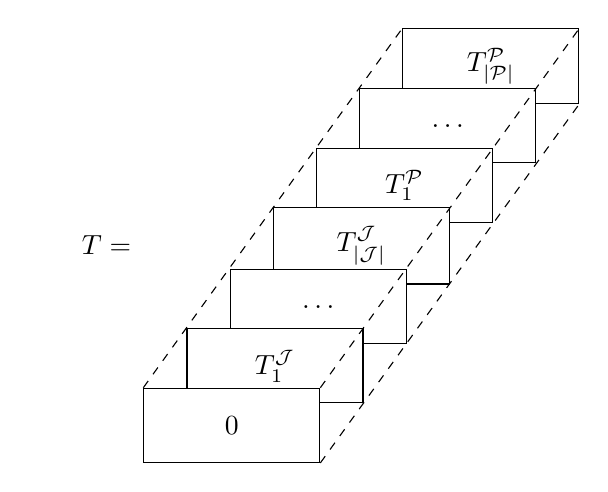
\begin{tikzpicture}[every node/.style={anchor=north east,fill=white,minimum width=2cm,minimum height=7mm}]
            
            % Define the displacement as a coordinate
            \coordinate (displacement) at (1.7,0.2);
        
            \matrix (mLP) [draw,matrix of math nodes]
                {
                T^\mcP_{|\mcP|} \\
                };
        
            \matrix (dots2) [draw,matrix of math nodes] at ($(mLP.south west)+(displacement)$)
                {
                \dots \\
                };
        
            \matrix (mLp) [draw,matrix of math nodes] at ($(dots2.south west)+(displacement)$)
                {
                T^\mcP_{1} \\
                };
        
            \matrix (mLJ) [draw,matrix of math nodes] at ($(mLp.south west)+(displacement)$)
                {
                T^\mcJ_{|\mcJ|} \\
                };
        
            \matrix (dots1) [draw,matrix of math nodes] at ($(mLJ.south west)+(displacement)$)
                {
                \dots \\
                };
        
            \matrix (mLj) [draw,matrix of math nodes] at ($(dots1.south west)+(displacement)$)
                {
                T^\mcJ_1 \\
                };

            \matrix (m0) [draw,matrix of math nodes] at ($(mLj.south west)+(displacement)$)
                {
                0 \\
                };
            
            \draw[dashed](m0.north east)--(mLP.north east);
            \draw[dashed](m0.north west)--(mLP.north west);
            \draw[dashed](m0.south east)--(mLP.south east);
            
            \node at ($(-5,-2.4)$) {$T=$};
            
            \end{tikzpicture}
        \end{equation}
    \end{minipage}
\end{center}
The structure of the storage matrix $\tilde{x}_{SSMO}$ is the same as $\tilde{x}_{3D}$ in \eqref{eqn:A-tilde-3D}. The selection of the final estimate follows the same procedure as described in Section \ref{subsec:estimate-selection}.

\begin{table}[h]
    \centering
    \begin{tabular}{c|c|c}
       Matrix  & Dimensions & Number of elements \\ \hline
       $\Tilde{x}_{SSMO}$  & $ n_x \times 1 \times N_S$ & $_xN_S$ \\
       $\mathbf{A}$ & $n_xN_O \times n_xN_O$ & $n_x^2N_O^2$ \\ 
       $\mathbf{B}$ & $n_xN_O \times n_x$ & $n_x^2N_O$ \\
       $T$ & $n_x \times n_xN_O \times N_S$ & $n_x^2N_ON_S$ \\
    \end{tabular}
    \caption{SSMO system matrix dimensions}
    \label{tab:SSMO-dimensions}
\end{table}

\subsection{Size comparison}
Let us now compare the sizes of the 2D-CMO, 3D-CMO and SSMO as presented in Tables \ref{tab:2D-CMO-dimensions}, \ref{tab:3D-CMO-dimensions} and \ref{tab:SSMO-dimensions} respectively. First, the total number of elements for each MO is derived from the matrices that are needed to construct it. 
\begin{table}[h]
    \centering
    \begin{tabular}{c|c}
        Multi-Observer & Total number of Elements \\
        \hline
        2D-CMO & $n_x^2N_S^2 + N_S(n_x+2n_u)$ \\
        3D-CMO & $n_xN_s(1+2n_x)$ \\
        SSMO   & $n_xN_S(1+n_xN_O) + n_x^2N_O(N_O+1)$ \\
    \end{tabular}
    \caption{Total number of elements in each MO implementation}
    \label{tab:my_label}
\end{table}

We now use the for $N_S$ as in equation \eqref{eqn:NS-approximation} to compare number of Gigabytes required to store the MO. The comparison is made for different combinations of the number of state variables $n_x$ and number of total system outputs $N_O$. Both of these values are ranged from $1$ to $100$ and the storage size for each combination is compared.

\begin{figure}
    \centering
    \includegraphics[width=0.5\linewidth]{size}
    \caption{Caption}
    \label{fig:enter-label}
\end{figure}
\newpage
\section{Matlab implementation}\label{ch:matlab-implementation}
Both CMOs and the SSMO as defined in Subsections \ref{subsec:CMO-architecture} and \ref{subsec:ssmo-architecture} have been implemented in Matlab. In this chapter the implementations will be discussed and the MOs will be applied on the mass-spring-damper system as described in Chapter \ref{ch:system-definition}. The implementation uses classes for the system, attack, shared multi-observers and the specific multi-observers. All of these will be discussed in this chapter, the code itself can be found in Appendix \ref{ap:matlab-code}.

\subsection{Class explanation}
The system class (\texttt{msd}) defines the system matrices for a mass-spring-damper as in Chapter \ref{ch:system-definition}. The class can creates the state-space system consisting of matrices \eqref{eqn:msd-A}\eqref{eqn:msd-B}\eqref{eqn:msd-E}\eqref{eqn:msd-C}. The class can create both linear and nonlinear systems and works for any number of masses in series.

The \texttt{attack} class defines an attack on the system, the outputs that are to be attacked can be specified. If no outputs are specified, a random selection is made. A list with ones indicating an attack and zeros indicating no attack is made, later on this one is substituted by the attack signal. The specific attack signal can be changed within the \texttt{attackFunction} function.

All MOs are based on a common set of $J$-observers and $P$-observers as defined in Subsection \ref{subsec:state-estimates}. Since all MOs observe the same system, these observers can be defined once and used by all MOs. A separate \texttt{mo} object needs to be generated for both the $J$ and $P$-observers. The \texttt{mo} defines observers for each combination as defined in \eqref{eqn:observer-sets}, based on a given number of outputs for each observer (size of each combination). The class generates an $L$ matrix that places the eigenvalues of $A + LC$ at specified locations. Usually, the size of $C$ does not match the number of outputs $N_O$. The \texttt{mo} class automatically creates a set of outputs based on the provided $C$ where the number of rows matches $N_O$.

\textcolor{red}{2D CMO}

The \texttt{cmo3d} class defines the 3D CMO based on the two \texttt{mo} objects for the $J$ and $P$-observers and the system. It generates the system matrices \eqref{eqn:x3d}\eqref{eqn:A-tilde-3D}\eqref{eqn:F-3d}\eqref{eqn:L-3d}\eqref{eqn:eta-3d} and uses the \texttt{attack} object to create a 3D attack vector that stores the ones and zeros for each specific observer.

The \texttt{ssmo} class defines the SSMO based on the \texttt{mo} objects. It generates the shared system matrices \eqref{eqn:controllable-canonical-form} and all transformation matrices \eqref{eqn:ssmo-transformation}. 

\subsection{Running a simulation}
All MOs can be simulated under the same conditions and the results can be compared. The file \texttt{mainClassScript.m} in Appendix \ref{ap:matlab-code}, generates all MOs and solves the ODEs as in equation \eqref{eqn:standard-system}, \eqref{eqn:cmo-single-J-observer} and \eqref{eqn:cmo-single-P-observer}. Figure \ref{fig:unattacked-system-plot} displays the solution of this ODE for the system as in Example \ref{ex:system}. The observer quickly approaches the system state and the error decays to zero.

\begin{figure}[ht]
    \centering
    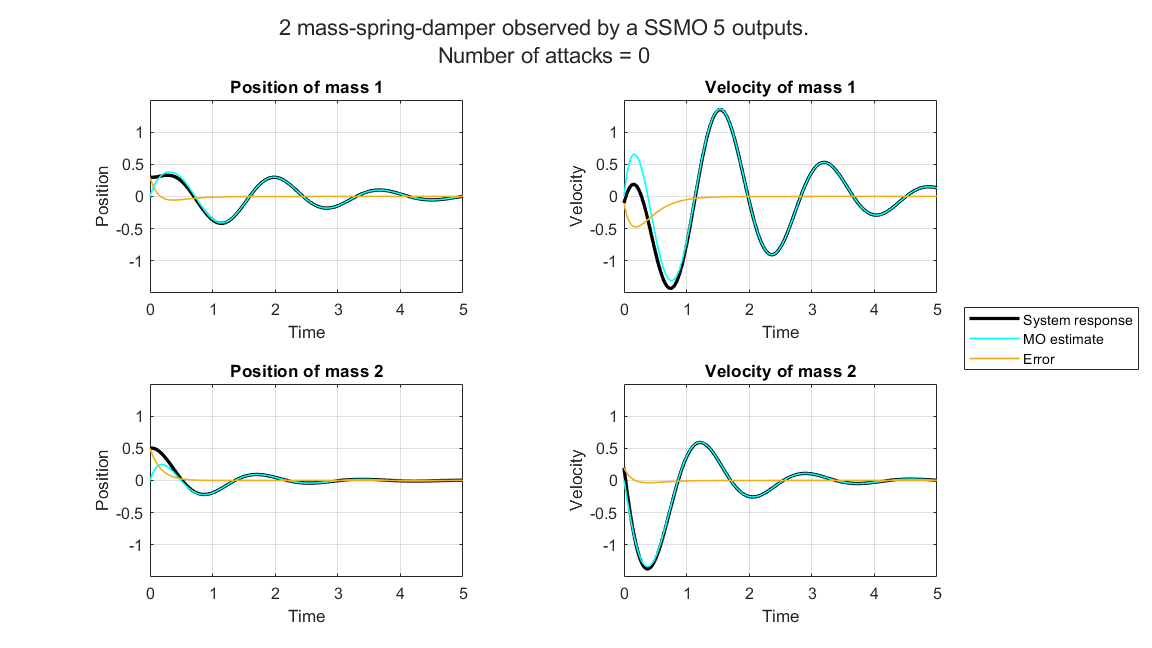
\includegraphics[width=\linewidth]{report/Figures/symplot_5o0a.png}
    \caption{An unattacked, noiseless double mass spring damper and an observer}
    \label{fig:unattacked-system-plot}
\end{figure}

Let us now introduce the attack as in Figure \ref{fig:attack-diagram}, so outputs 2 and 5 are under attack. The attack signal $\tau_j=t,j=2,5$ is injected into both outputs. 

\begin{figure}
    \centering
    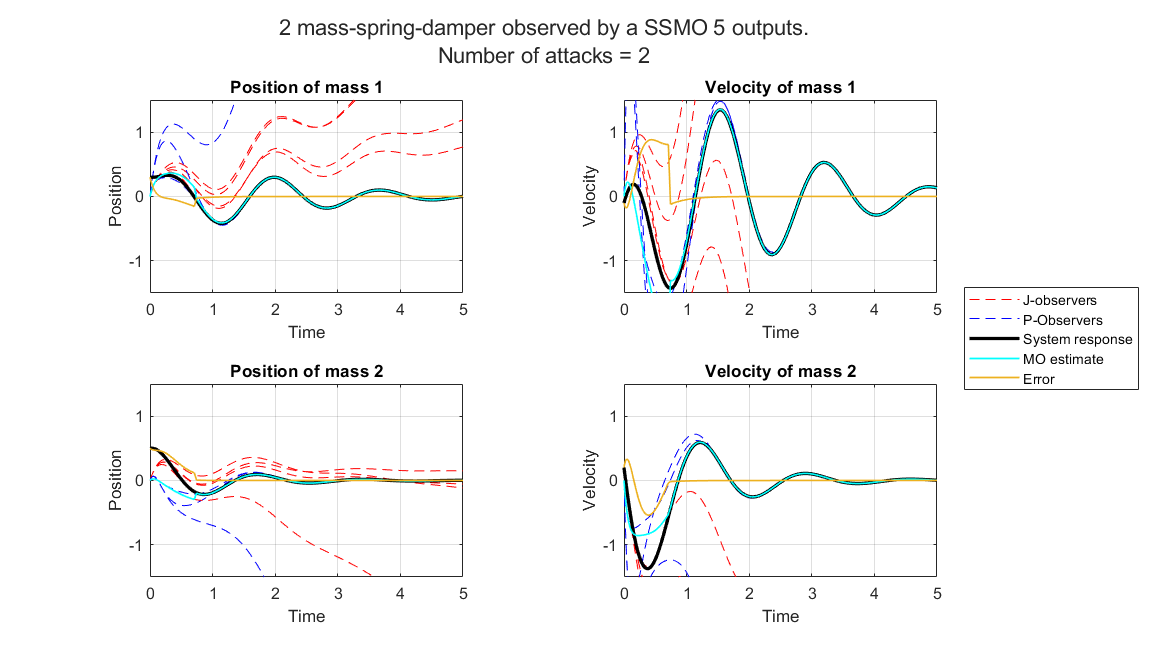
\includegraphics[width=\linewidth]{report/Figures/symplot_5o2a}
    \caption{Caption}
    \label{fig:enter-label}
\end{figure}
\newpage
\section{Nonlinear multi-observers}\label{ch:nonlinear-mos}
In this chapter the issues with MOs applied on nonlinear systems will be discussed. We will employ an MO on system \eqref{eqn:standard-system} which will be repeated here for clarity
\begin{equation*}
    \begin{split}
        \dot{x}(t) &= Ax(t) + Bu(t) + E\phi(x) \\
        y_i(t) &= C_ix(t) + Du(t) + v_i(t) + \tau_i(t) \quad i \in \mathcal{N} = \{1,2,\dots,N_O\}.
    \end{split}
\end{equation*}
First the observers will be extended with the aim of correctly observing the state of system \eqref{eqn:standard-system} when less then half of the sensors are under attack (the same boundary condition as discussed in Chapter \ref{ch:cmo}).

\subsection{Extending the state-estimates}
Let us extend the MO to also observe nonlinear systems as a single observer in Equation \eqref{eqn:nonlinear-single-observer}. Let us extend the observers as in Equations \eqref{eqn:cmo-single-J-observer}
\begin{equation}\label{eqn:nonlinear-mo}
    \begin{split}
        \dot{\hat{x}}_{j/p}^{\mcJ/\mcP} &= (A + L_{j/p}^{\mcJ/\mcP}C_{j/p}^{\mcJ/\mcP})\hat{x}^{\mcJ/\mcP}_{j/p} - L_{j/p}^JC_{j/p}^{\mcJ/\mcP}x + Bu + E\phi(y) - L_{j/p}^{\mcJ/\mcP}(v_{j/p}^{\mcJ/\mcP} + \tau_{j/p}^{\mcJ/\mcP}),
    \end{split}
\end{equation}
where $j=1,2,\dots,N_J$, $p=1,2,\dots,N_P$ and $j/p$ indicates that the equation holds for both $J$ and $P$-observers. The resulting observer in Equation \ref{eqn:nonlinear-mo} is analogous to the observer in \cite[Equation 5]{Chong2023MemoryAlgorithms}. In this case the nonlinearity is output dependent, the full $y$ is used as input and not the subset that corresponds to the the specific $p$ or $j$. This has some implications in the SSE context, where some $y_i$ are corrupted. If the $y_i$ that happen to be used by the nonlinearity $\phi(y)$ is attacked, all state estimates become corrupted. So no 

\begin{example}\label{ex:nonlinear-issue}
    Let us work through an example to clarify this issue, consider system \eqref{eqn:example-system} as defined in Example \ref{ex:system}, where we change $C$ to have $N_O=6$ outputs
    \begin{equation}\label{eqn:NL-ex-C-6out}
        C = 
        \begin{bmatrix}
            1 & 0 & 0 & 0 \\
            1 & 0 & 1 & 0 \\
            1 & 0 & 0 & 0 \\
            1 & 0 & 1 & 0 \\
            1 & 0 & 0 & 0 \\
            1 & 0 & 1 & 0 \\
        \end{bmatrix}.
    \end{equation}
    This means there are 3 copies of each sensor. The nonlinear spring as in Equation \eqref{eqn:nonlinear-spring} uses the spring constants and positions of each individual mass as input. Since we now have three copies of each position sensor we can select any combination of two sensors measuring a different position. Let us select the first two sensors, $y_1$ and $y_2$. We now construct
    \begin{equation}\label{eqn:NL-ex-phi-6out}
        \phi(y) = 
        \begin{bmatrix}
            F^{NL}_s(y_1) \\ F^{NL}_s(y_2) \\
        \end{bmatrix},
    \end{equation}
    which leads to the following $E$ matrix
    \begin{equation}\label{eqn:NL-ex-E-6out}
        E =
        \begin{bmatrix}
            0 & 0 \\
            -1 & 1 \\
            0 & 0 \\
            0 & -1 \\
        \end{bmatrix}.
    \end{equation}
    Figure \ref{fig:nonlinear-functional} displays a scenario where $\mathcal{M}=\{3,6\}$, so outputs $3$ and $6$ are under attack, with the attack signal $\tau_k=t,k \in \mathcal{M}$ The MO works as expected and provides a correct state estimate. The $\phi(y)$ provides a correct value for all $t \geq 0$.
    \begin{figure}[H]
        \centering
        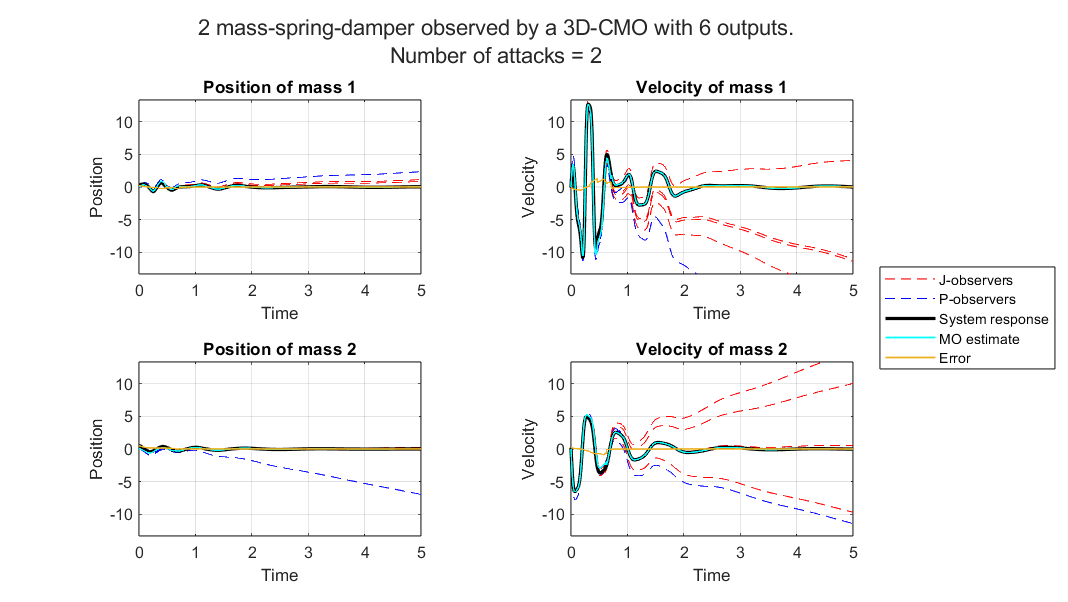
\includegraphics[width=\linewidth]{report/Figures/nonlinear_functional.png}
        \caption{Nonlinear double mass-spring-damper model with outputs $3$ and $6$ under attack.}
        \label{fig:nonlinear-functional}
    \end{figure}
    Figure \ref{fig:nonlinear-not-functional} shows a scenario where $\mathcal{M}=\{1,4\}$. Or in other words, outputs $1$ and $4$ are under attack. The attack signal is the same as in the previous case, $\tau_k=t,k \in \mathcal{M}$. All state estimates fail in this case, because $\phi(y)$ uses an attacked output.

    \begin{figure}[H]
        \centering
        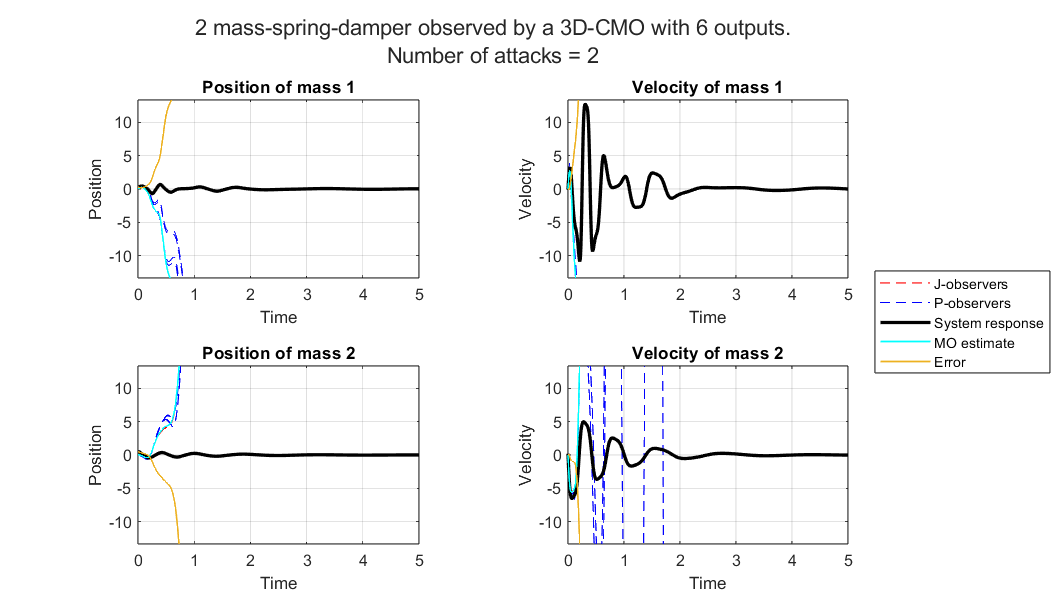
\includegraphics[width=\linewidth]{report/Figures/nonlinear_not_functional.png}
        \caption{Nonlinear double mass-spring-damper model with outputs $1$ and $4$ under attack.}
        \label{fig:nonlinear-not-functional}
    \end{figure}
\end{example}

Both Figures \ref{fig:nonlinear-functional} and \ref{fig:nonlinear-not-functional} show the result of a 3D-CMO, the result on an SSMO is the same. Not surprising, since they realize the same set of observers.

\subsection{Addressing the nonlinear issue}
As discussed in Example \ref{ex:nonlinear-issue} the issue arises because the observers' nonlinear extension does not employ any intelligent logic in choosing which outputs are used to calculate the nonlinear contribution. The nonlinearity $\phi(y)$ should either 'know' which $y_i$ are corrupted and avoid them, which is contradictory with the demands of SSE. Or it should be able to provide a correct state estimate even with an unknown subset of sensors under attack. Let us now discuss the implications and difficulties of this issue for both the 3D-CMO and the SSMO, we will not consider the 2D-CMO in this section. 

Let us start with the SSMO, the shared state is calculated as in Equation \eqref{eqn:ssmo-z} which we repeat for readability
\begin{equation*}
    \dot{z} = \mathbf{A}z + \mathbf{B}\eta, \quad \eta = 
    \begin{bmatrix}
        u \\ y
    \end{bmatrix}.
\end{equation*}
The nonlinearity no longer appears in this structure, since it is taken into account during construction of the shared $\mathbf{B}$ matrix. The input to the nonlinear function $\phi(y)$ is also 'hidden' behind the shared state. We cannot try different combinations of sensors $y_i$ because we only calculate a single state $z$, which uses a single external input $\eta$ with the full output $y$.

We now continue with the 3D-CMO, which has more control over each individual state estimate $\hat{x}^{\mcJ/\mcP}_{j/p}$. Since every observer is calculated separately, a different nonlinear contribution can be used for every observer
\begin{equation}\label{eqn:ext-NL-observer}
    \begin{split}
        \dot{\hat{x}}_{j/p}^{\mcJ/\mcP} &= (A + L_{j/p}^{\mcJ/\mcP}C_{j/p}^{\mcJ/\mcP})\hat{x}^{\mcJ/\mcP}_{j/p} - L_{j/p}^JC_{j/p}^{\mcJ/\mcP}x + Bu + E\phi(y^{\mcJ/\mcP}_{j/p}) - L_{j/p}^{\mcJ/\mcP}(v_{j/p}^{\mcJ/\mcP} + \tau_{j/p}^{\mcJ/\mcP}).
    \end{split}
\end{equation}
The nonlinear contribution $E\phi(y^{\mcJ/\mcP}_{j/p})$ uses the subset $j$ or $p$ as input to the function $\phi(y)$. Let us work out two examples that clarify some of the implications this extended 3D-CMO has. We start with an example that investigates a system where $\phi(y)$ is dependent only on one measured state variable.

\begin{example}\label{ex:single-mass-nonlinear-example}
    Consider the system as in Equation \eqref{eqn:standard-system} with system matrices
    \begin{equation*}
        A =
        \begin{bmatrix}
            0 & 1 \\ -15 & -2 \\
        \end{bmatrix}, \quad
        B =
        \begin{bmatrix}
            0 \\ 1 \\
        \end{bmatrix}, \quad
        C = 
        \begin{bmatrix}
            1 & 0 \\ 1 & 0 \\ 1 & 0 \\ 1 & 0 \\ 1 & 0 \\
        \end{bmatrix}, \quad
        D = 0, \quad
        E =
        \begin{bmatrix}
            0 \\ -1 \\
        \end{bmatrix},   
    \end{equation*}
    as derived from the general mass-spring-damper described in Chapter \ref{ch:system-definition}.  The nonlinearity looks like
    \begin{equation*}
        \phi(y^{\mcJ/\mcP}_{j/p}) = F^{NL}_s((y^{\mcJ/\mcP}_{j/p})_1),
    \end{equation*}
    where the subscript $1$ indicates the first element of $y^{\mcJ/\mcP}_{j/p}$. The system has $N_O=5$ outputs, let us attack $N_M=2$ of those outputs. $\mathcal{M}=\{2,4\}$, so outputs $2$ and $4$ are under attack. Again the attack signal $\tau_k=t,k \in \mathcal{M}$ is used. Figure \ref{fig:single-nonlinear-functional} shows the result of such an attack, the MO successfully estimates the state and the error approaches zero. 
    \begin{figure}[H]
        \centering
        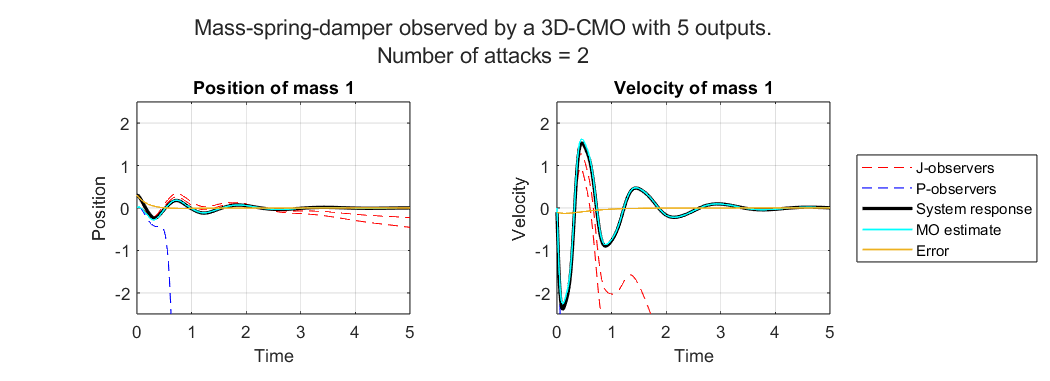
\includegraphics[width=\linewidth]{report/Figures/single-nonnlinear-functional.png}
        \caption{Single nonlinear mass-spring-damper with outputs $2$ and $4$ under attack.}
        \label{fig:single-nonlinear-functional}
    \end{figure}
    In this scenario the MO functions because all sensors measure the same variable, the position of the first (and only) mass. So the combination $j=\{1,3,5\}$ provides a successful state estimate because $\phi(y_1)=\phi(y_3)=\phi(y_5)=\phi(\begin{bmatrix}y_1&y_3&y_5\end{bmatrix}^T)$. 
\end{example}
Let us now investigate a scenario where the nonlinearity $\phi(y)$ depends on multiple measured state variables.

\begin{example}\label{ex:ext-NL-double-mass}
    Now, consider the same system \eqref{eqn:example-system} as in Example \ref{ex:system}, where $C$ is changed to have $N_O=5$
    \begin{equation*}
        C = 
        \begin{bmatrix}
            1 & 0 & 0 & 0 \\
            1 & 0 & 1 & 0 \\
            1 & 0 & 0 & 0 \\
            1 & 0 & 1 & 0 \\
            1 & 0 & 0 & 0 \\
        \end{bmatrix}.
    \end{equation*}
    Let us now choose $N_M=2$ in order to still satisfy the $N_O>2N_M$ requirement. Where we specify $\mathcal{M}$ as $\{2,4\}$, note that now all copies of the sensor measuring the position of mass 2 are attacked. Figure \ref{fig:extended_nonlinear_not_functional} shows that the error $\hat{x}-x$ still approaches $0$ as $t$ increases. But the estimates, especially of the velocities, do not look to be tracking the true state correctly.
    \begin{figure}[H]
        \centering
        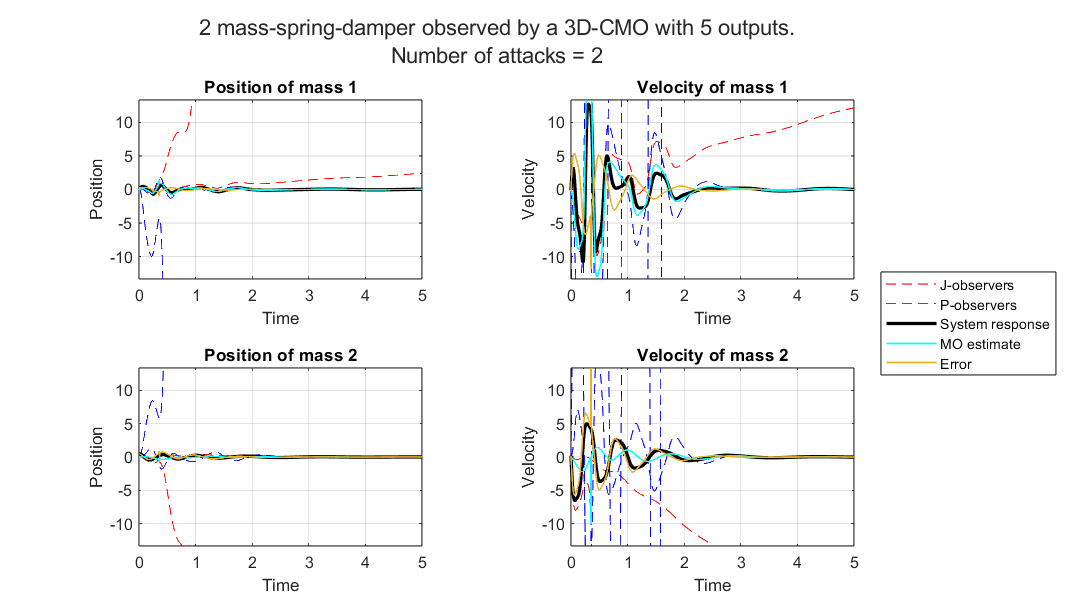
\includegraphics[width=\linewidth]{report/Figures/extended_nonlinear_not_functional.png}
        \caption{Double nonlinear mass-spring-damper with outputs 2 and 4 under attack.}
        \label{fig:extended_nonlinear_not_functional}
    \end{figure}
    Let us now expand the number of outputs to $N_O=6$, and use the exact same system as in Equations \eqref{eqn:NL-ex-C-6out},\eqref{eqn:NL-ex-E-6out} and \eqref{eqn:NL-ex-phi-6out} as in Example \ref{ex:nonlinear-issue}. We now use the observer as in Equation \eqref{eqn:ext-NL-observer} and attack the system with the attack signal $\tau_k=t,k \in \mathcal{M},\mathcal{M}=\{4,6\}$ \textcolor{red}{ugly}.
    \begin{figure}[H]
        \centering
        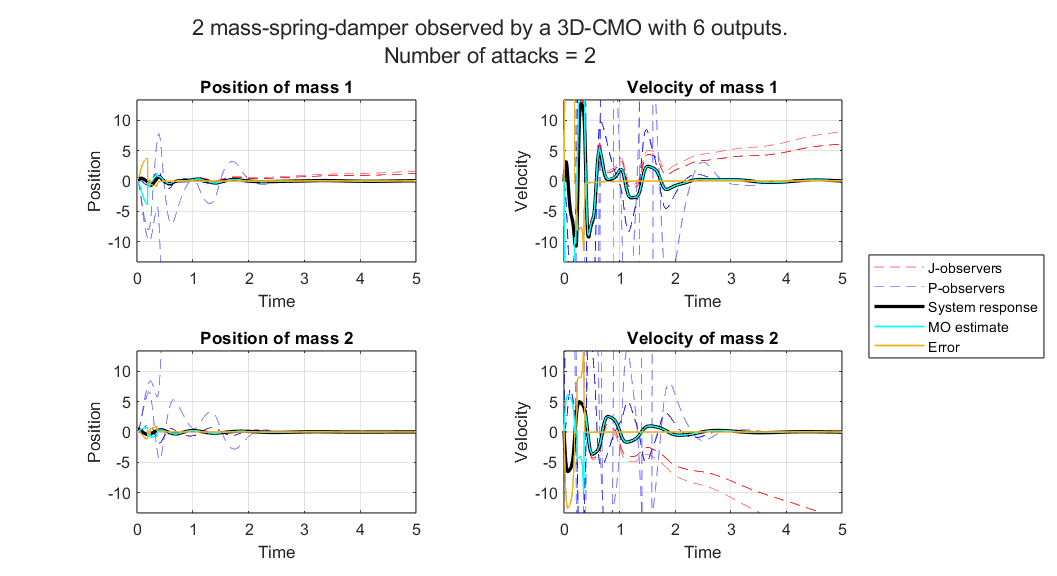
\includegraphics[width=\linewidth]{report/Figures/extended-nonlinear-functional.png}
        \caption{Double mass-spring-damper with outputs $4$ and $6$ under attack.}
        \label{fig:extended-nonlinear-functional}
    \end{figure}
    The state estimates in Figure \ref{fig:extended-nonlinear-functional} look to be tracking the true state much better. The MO now functions correctly because the state estimate using $j=\{1,2,3,5\}$ has the uncorrupted outputs $1$ and $2$ as input to $\phi(y)$ as in Equation \eqref{eqn:NL-ex-phi-6out}.
\end{example}
The attacked outputs in Example \ref{ex:ext-NL-double-mass} have, of course, been carefully chosen to provide the correct results. Had we attacked outputs $2$ and $4$ in the $N_O=6$ case, no correct state estimate could have been provided. This happens because in the setup in the example $\phi(y)$ takes the first two entries of $y^{\mcJ/\mcP}_{j/p}$ irrespective of what the sensor measures. So if outputs $2$ and $4$ are attacked, even the fully uncorrupted set of outputs $j=\{1,3,5,6\}$ does not provide a correct state estimate. Because $\phi(y)$ is only considers outputs $1$ and $3$ in this state estimate. If we provide the reading of sensor $6$ in the second position, the nonlinearity would use the correct input value. For a double mass-spring-damper system the outputs could be sorted to feature uneven and even sensors in an alternating pattern, as long as possible. For the set we are considering now, it could take the form $\{1,6,3,5\}$ \textcolor{red}{how to denote ordered sets?}. In order to generalize this method for systems with a nonlinearity depending on $n$ variables the list should be sorted based on multiples... \textcolor{red}{if this stays in needs to much more detailed}

Up till now, only the $J$-observers have been discussed. Let us use the set of outputs $j=\{1,3,5,6\}$ again. During the final estimate selection procedure as described in subsection \ref{subsec:estimate-selection}. All estimates constructed with $p \in j$ are compared against the estimate constructed with $j$. We now encounter the same pitfall as before: for all sizes of $p$ that are smaller then $|j|$, some possible subsets do not contain any sensor measuring the position of the second mass.
\newpage
\section{Conclusion}
This BEP has implemented three multi-observer variants and compared them based on memory usage. The 2D-CMO and the 3D-CMO store all state estimates individually, where 3D-CMO is much more memory efficient as compared to the 2D-CMO. Unlike the CMOs, the SSMO condenses all observers into a single state. In order to perform the final estimate selection procedure the original states are still required. These are recovered through transformation matrices. Although the shared state of the SSMO requires much less memory than all the individual states of the CMOs, the transformation matrices used to recover the original states still requires significant memory. 

In a direct comparison between the 2D-CMO, 3D-CMO and the SSMO, the 3D-CMO uses the least memory. It should be noted that the 3D-CMOs memory requirements are still significantly too large for an implementation in a system with a large number of outputs.

The MOs extension to observe nonlinear systems remains incomplete, creating aggregate sensors seems to be a promising solution to the issues presented in this BEP. Although the SAMO seems to function well under the tested circumstances, no statements have been made about its implementation on general systems. The LAMO does not show immediate improvements over the SAMO.

Let us note several limitations of this BEP. The size comparison between multiple linear MOs does not consider systems with $P$-observers using a size larger than 1, selecting a different value can be required in order to properly observe a system. This could cause a different total MO size, although the size differences between the MO implementations are believed to be similar. This report has not considered MOs observing a system while feedback control is applied to the system and no effort has been made to select observer eigenvalues based on noise rejection and fast error suppression. Implementing feedback control could require changes to the structure of the CMO in order to select the desired eigenvalues. The Matlab implementations themselves have become overcomplicated in order to run the observers simultaneously.

In order to make a real-world MO implementation possible, more effort needs to be put in reducing the required memory. There is also still a need for further research into the nonlinear extension of the 3D-CMO, the feasibility of the SAMO is questionable regarding the increased size as compared to a linear MO. The unexplained behaviour of the LAMO could be key to expanding the functionality beyond the limit of the attacked aggregate sensors. Although it is also possible that it can never guarantee a secure state estimate beyond this limit.

\newpage
\bibliographystyle{plain}
\bibliography{report/references.bib}

\newpage
\begin{appendices}

\section{Stirling's approximation}
\begin{table}[ht]
\centering
\begin{tabular}{|c|c|c|}
\toprule
\textbf{n} & \textbf{Exact Factorial} & \textbf{Stirling's Approximation} \\ \midrule
1 & $1$ & $0.9221$ \\
2 & $2$ & $1.9190$ \\
3 & $6$ & $5.8362$ \\
4 & $24$ & $23.5062$ \\
5 & $120$ & $118.0192$ \\
6 & $720$ & $710.0782$ \\
7 & $5040$ & $4.9804 \times 10^3$ \\
8 & $40320$ & $3.9902 \times 10^4$ \\
9 & $362880$ & $3.5954 \times 10^5$ \\
10 & $3628800$ & $3.5987 \times 10^6$ \\
11 & $39916800$ & $3.9616 \times 10^7$ \\
12 & $479001600$ & $4.7569 \times 10^8$ \\
13 & $6.2270 \times 10^9$ & $6.1872 \times 10^9$ \\
14 & $8.7178 \times 10^{10}$ & $8.6661 \times 10^{10}$ \\
15 & $1.3077 \times 10^{12}$ & $1.3004 \times 10^{12}$ \\
16 & $2.0923 \times 10^{13}$ & $2.0814 \times 10^{13}$ \\
17 & $3.5569 \times 10^{14}$ & $3.5395 \times 10^{14}$ \\
18 & $6.4024 \times 10^{15}$ & $6.3728 \times 10^{15}$ \\
19 & $1.2165 \times 10^{17}$ & $1.2111 \times 10^{17}$ \\
20 & $2.4329 \times 10^{18}$ & $2.4228 \times 10^{18}$ \\
\bottomrule
\end{tabular}
\caption{Comparison of Exact Factorial and Stirling's Approximation}
\label{tab:factorial_stirling}
\end{table}

\newpage
\section{SSMO transformation matrix}\label{ap:ssmo-transformation-matrix}
Let us now show that the transformation matrix $T_o=R_pR_q$,
\begin{equation*}
    \begin{split}
         R_p &=
        \begin{bmatrix}
            \B_o & \A_o\B_o & \A^{2}_o\B_o & \cdots & \A^{n-1}_o\B_o \\
        \end{bmatrix} \\
        R_q &=
        \begin{bmatrix}
            I_l & q_1I_l & q_2I_l & \cdots & q_{n-1}I_l \\
            0_l & I_l & q_1I_l & \cdots & q_{n-2}I_l \\
            \vdots & \ddots & \ddots & \ddots & \vdots \\
            0_l & \cdots & 0_l & I_l & q_1I_l \\
            0_l & \cdots & 0_l & 0_l & I_l \\
        \end{bmatrix}.
    \end{split}
\end{equation*}
transforms the system \eqref{eqn:ssmo-standard-system-form} into controllable canonical form as in Equation \eqref{eqn:controllable-canonical-form}, with the transformation
\begin{equation}\label{eqn:A-transformation}
    \begin{split}
        T_o\mathbf{A} &= \A_oT_o \\
        R_pR_q\mathbf{A} &= \A_oR_pR_q. \\
    \end{split}
\end{equation}
 Let us start by expanding
\begin{equation*}
    \begin{split}
        R_q\mathbf{A} &=  
        \begin{bmatrix}
            I_l & q_1I_l & q_2I_l & \cdots & q_{n-1}I_l \\
            0_l & I_l & q_1I_l & \cdots & q_{n-2}I_l \\
            \vdots & \ddots & \ddots & \ddots & \vdots \\
            0_l & \cdots & 0_l & I_l & q_1I_l \\
            0_l & \cdots & 0_l & 0_l & I_l \\
        \end{bmatrix}
        \begin{bmatrix}
            -q_1I_l & -q_2I_l & \cdots & -q_{n-1}I_l & -q_nI_l \\
            I_l & 0_l & \cdots & 0_l & 0_l \\
            0_l & I_l & \cdots & 0_l & 0_l \\
            \vdots & \vdots & \ddots & \vdots & \vdots \\
            0_l & 0_l & \cdots & I_l & 0_l \\
        \end{bmatrix} \\
        &= 
        \begin{bmatrix}
            0_l & 0_l & 0_l & \cdots & 0_l & 0_l & 0_l \\
            I_l & q_1I_l & q_2I_l & \cdots & q_{n-3}I_l & q_{n-2}I_l & 0_l \\ 
            0_l & I_l & q_1I_l & \cdots & q_{n-4}I_l & q_{n-3}I_l & 0_l \\ 
            \vdots & \vdots & \vdots & \ddots & \vdots & \vdots & \vdots \\
            0_l & 0_l & 0_l & \cdots & q_1I_l & q_2I_l & 0_l \\
            0_l & 0_l & 0_l & \cdots & I_l & q_1I_l & 0_l \\
            0_l & 0_l & 0_l & \cdots & 0_l & I_l & 0_l \\
        \end{bmatrix}.
    \end{split} 
\end{equation*}
We now premultiply this by $R_o$
\begin{equation*}
    \begin{split}
        R_pR_q\mathbf{A} &= 
        \begin{bmatrix}
            \B_o & \A_o\B_o & \A^{2}_o\B_o & \cdots & \A^{n-1}_o\B_o \\
        \end{bmatrix}
        \begin{bmatrix}
            0_l & 0_l & 0_l & \cdots & 0_l & 0_l \\
            I_l & q_1I_l & q_2I_l & \cdots & q_{n-2}I_l & 0_l \\ 
            0_l & I_l & q_1I_l & \cdots & q_{n-3}I_l & 0_l \\ 
            \vdots & \ddots & \ddots & \ddots & \vdots & \vdots \\
            0_l & 0_l & 0_l & \ddots & q_1I_l & 0_l \\
            0_l & 0_l & 0_l & \cdots & I_l & 0_l \\
        \end{bmatrix} \\
        &= 
        \begin{bmatrix}
            \A_o\B_o \\ q_1\A_o\B_o + \A^2_o\B_o \\ q_2\A_o\B_o + q_1\A^2_o\B_o + \A^3_o\B_o \\ \cdots \\ q_{n-2}\A_o\B_o + q_{n-3}\A^2_o\B_o + \cdots + q_1\A^{n-2}_o\B_o + \A^{n-1}_o\B_o \\ 0 \\      
        \end{bmatrix}^T
    \end{split}
\end{equation*}
Where by the Cayley-Hamilton theorem we can rewrite penultimate column as
\begin{equation*}
    \begin{bmatrix}
            \A_o\B_o \\ q_1\A_o\B_o + \A^2_o\B_o \\ q_2\A_o\B_o + q_1\A^2_o\B_o + \A^3_o\B_o \\ \vdots \\ -\A^n_o\B_o \\ 0 \\      
        \end{bmatrix}^T
\end{equation*}

We now expand
\begin{equation*}
    \begin{split}
        \A_oR_pR_q &= 
        \begin{bmatrix}
            \A_o\B_o & \A^2_o\B_o & \A^{3}_o\B_o & \cdots & \A^{n}_o\B_o \\
        \end{bmatrix}
        \begin{bmatrix}
            I_l & q_1I_l & q_2I_l & \cdots & q_{n-1}I_l \\
            0_l & I_l & q_1I_l & \cdots & q_{n-2}I_l \\
            \vdots & \ddots & \ddots & \ddots & \vdots \\
            0_l & \cdots & 0_l & I_l & q_1I_l \\
            0_l & \cdots & 0_l & 0_l & I_l \\
        \end{bmatrix} \\
        &=
        \begin{bmatrix}
            \A_o\B_o \\ 
            q_1\A_o\B_o + \A^2_o\B_o \\ 
            q_2\A_o\B_o + q_1\A^2\B_o + \A^3_o\B_o \\ \vdots \\ 
            q_{n-1}\A_o\B_o + q_{n-2}\A^2_o\B_o + \cdots + \A^{n-1}_o\B_o \\
            q_{n-1}\A_o\B_o + q_{n-2}\A^2_o\B_o + \cdots + \A^{n-1}_o\B_o + \A^n_o\B_o \\
        \end{bmatrix}^T,
    \end{split}
\end{equation*}
where the bottom two rows can be simplified by using the Cayley-Hamilton theorem
\begin{equation*}
    \begin{split}
        \A_oR_pR_q &= 
        \begin{bmatrix}
            \A_o\B_o \\ 
            q_1\A_o\B_o + \A^2_o\B_o \\ 
            q_2\A_o\B_o + q_1\A^2\B_o + \A^3_o\B_o \\ \vdots \\ 
            \A^{n}_o\B_o \\
            0 \\
        \end{bmatrix}^T,
    \end{split}
\end{equation*}
which is equal to $R_oR_q\A_o$. We can now conclude that the matrix $T_o=R_oR_q$ satisfies \eqref{eqn:A-transformation}. Now we will show the same for
\begin{equation}\label{eqn:B-transformation}
    \begin{split}
        T_o\mathbf{B} &= \B_o \\
        R_pR_q\mathbf{B} &= \B_o.
    \end{split}
\end{equation}
Let us expand
\begin{equation*}
    \begin{split}
        R_pR_q\mathbf{B} &=
        \begin{bmatrix}
            \B_o & \A_o\B_o & \A^{2}_o\B_o & \cdots & \A^{n-1}_o\B_o \\
        \end{bmatrix}
        \begin{bmatrix}
            I_l & q_1I_l & q_2I_l & \cdots & q_{n-1}I_l \\
            0_l & I_l & q_1I_l & \cdots & q_{n-2}I_l \\
            \vdots & \ddots & \ddots & \ddots & \vdots \\
            0_l & \cdots & 0_l & I_l & q_1I_l \\
            0_l & \cdots & 0_l & 0_l & I_l \\
        \end{bmatrix}
        \begin{bmatrix}
            I_l \\ 0_l \\ \vdots \\ 0_l \\ 0_l \\
        \end{bmatrix} \\
        &=
        \begin{bmatrix}
            \B_o & \A_o\B_o & \A^{2}_o\B_o & \cdots & \A^{n-1}_o\B_o \\
        \end{bmatrix}
        \begin{bmatrix}
            I_l \\ 0_l \\ \vdots \\ 0_l \\ 0_l \\
        \end{bmatrix} = \B_o \\
    \end{split}
\end{equation*}
which shows that \eqref{eqn:B-transformation} holds.

\newpage
\section{Matlab code Chapter \ref{ch:state-estimation}}\label{ap:matlab-code-ch3}
\lstinputlisting[style=Matlab-editor,caption=jordan$\_$form.m]{conventional/jordan_form.m}

\newpage
\section{Matlab code Chapter \ref{ch:cmo}}\label{ap:matlab-code-ch6}
\lstinputlisting[style=Matlab-editor,caption=sizeComparison.m]{conventional/sizeComparison.m}

\newpage
\section{Matlab code Chapter \ref{ch:matlab-implementation}}\label{ap:matlab-code}
Firstly, the main scripts is shown. This is the script than should be executed to run the model. Secondly, all classes are shown and finally all functions are shown. The documentation that sits between the function definitions and the start of the code are made by inputting the full function into ChatGPT-4 and with the prompt: "Can you provide documentation for this function? $<$code in between these brackets$>$" All output has been checked and corrected by the author in this report, so that the documentation accurately describes the code.
\lstinputlisting[style=Matlab-editor,caption=mainClassScript.m]{conventional/mainClassScript.m}
Now all classes follow alphabetically
\lstinputlisting[style=Matlab-editor,caption=attack.m]{functions/attack.m}
\lstinputlisting[style=Matlab-editor,caption=cmo2d.m]{functions/cmo2d.m}
\lstinputlisting[style=Matlab-editor,caption=cmo3d.m]{functions/cmo3d.m}
\lstinputlisting[style=Matlab-editor,caption=ssmo.m]{functions/ssmo.m}
\lstinputlisting[style=Matlab-editor,caption=mo.m]{functions/mo.m}
\lstinputlisting[style=Matlab-editor,caption=msd.m]{functions/msd.m}

Now all functions follow alphabetically
\lstinputlisting[style=Matlab-editor,caption=ApLCSetup.m]{functions/ApLCSetup.m}
\lstinputlisting[style=Matlab-editor,caption=attackFunction.m]{functions/attackFunction.m}
\lstinputlisting[style=Matlab-editor,caption=CNSetup.m]{functions/CNSetup.m}
\lstinputlisting[style=Matlab-editor,caption=CsetSetup.m]{functions/Csetsetup.m}
\lstinputlisting[style=Matlab-editor,caption=defineObservers.m]{functions/defineObservers.m}
\lstinputlisting[style=Matlab-editor,caption=etaSetup.m]{functions/etaSetup.m}
\lstinputlisting[style=Matlab-editor,caption=findIndices.m]{functions/findIndices.m}
\lstinputlisting[style=Matlab-editor,caption=flatten.m]{functions/flatten.m}
\lstinputlisting[style=Matlab-editor,caption=generateCombination.m]{functions/generateCombination.m}
\lstinputlisting[style=Matlab-editor,caption=inputDialog.m]{functions/inputDialog.m}
\lstinputlisting[style=Matlab-editor,caption=isMatrixStable.m]{functions/isMatrixStable.m}
\lstinputlisting[style=Matlab-editor,caption=isMemberOf.m]{functions/isMemberOf.m}
\lstinputlisting[style=Matlab-editor,caption=isObsv.m]{functions/isObsv.m}
\lstinputlisting[style=Matlab-editor,caption=isSubsetOf.m]{functions/isSubsetOf.m}
\lstinputlisting[style=Matlab-editor,caption=MOplot.m]{functions/MOplot.m}
\lstinputlisting[style=Matlab-editor,caption=multiObserverODE]{functions/multiObserverODE.m}
\lstinputlisting[style=Matlab-editor,caption=NLspring.m]{functions/NLspring.m}
\lstinputlisting[style=Matlab-editor,caption=pad3DL.m]{functions/pad3DL.m}
\lstinputlisting[style=Matlab-editor,caption=padL.m]{functions/padL.m}
\lstinputlisting[style=Matlab-editor,caption=rootsToCoefficients.m]{functions/rootsToCoefficients.m}
\lstinputlisting[style=Matlab-editor,caption=sbeCPU.m]{functions/sbeCPU.m}
\lstinputlisting[style=Matlab-editor,caption=selectRandomSubset.m]{functions/selectRandomSubset.m}
\lstinputlisting[style=Matlab-editor,caption=SSMOTransformationSetup.m]{functions/SSMOTransformationSetup.m}
\lstinputlisting[style=Matlab-editor,caption=systemPSetup.m]{functions/systemPSetup.m}
\lstinputlisting[style=Matlab-editor,caption=x0setup.m]{functions/x0setup.m}

\section{Matlab code chapter 7}\label{ap:matlab-code-ch7}
\lstinputlisting[style=Matlab-editor,caption=probabilities.m]{conventional/probabilities.m}
\end{appendices}

\end{document}

